%!TEX root=../../main.tex


\subsection{The frameworks during setup and benchmark}
We would like to raise some issues we encountered first while installing and configuring and second while running the different frameworks.

\begin{enumerate}
	\item During setup and benchmark of Gemini, we encountered several bugs in the cloned repository. These include non zero-terminated strings or even missing return statements.

	The errors rendered the code as-is unable to perform calculations, forcing us to fork the repository and modify the source code. A repository with our changes can be found \href{https://github.com/jasc7636/GeminiGraph}{here}\footnote{\url{https://github.com/jasc7636/GeminiGraph}}.

	\item Furthermore, we would like to address the setup of Hadoop for Giraph. It requires multiple edits in \texttt{xml} files that aren't easily automized. This makes the setup rather time consuming, especially if reconfiguration is needed later on.
	\item In order for Giraph to run, several Java tasks (the Hadoop infrastructure) have to be constantly running in the background. While we don't expect this to have a significant performance impact on other tasks, it is still suboptimal.
	%\item The Hadoop distributed file system (HDFS) ran us into disk space problems on multiple occasions. First, unless configured otherwise, the standard implementation replicates all data three times, distributed over all participating nodes. Second, deleting files on the HDFS does not immediately free up disk space because the files are moved to a \emph{recycling bin}-like location.

	\item 
\end{enumerate}


On a plus side, setup of frameworks like Polymer or Ligra was straight forward and did not require any special treatment. 


\subsection{Single-source Shortest-paths}
\autoref{fig:singleNodeSSSP} shows the average calculation times (time without initialization overhead), execution time and the normalized overhead for SSSP on the different frameworks. In these figures, Galois with 96 threads is shown. We show the impact of Galois' thread count in \autoref{sec:galois_speedup}.
\begin{figure*}[t!]
	\begin{subfigure}{0.3\textwidth}
		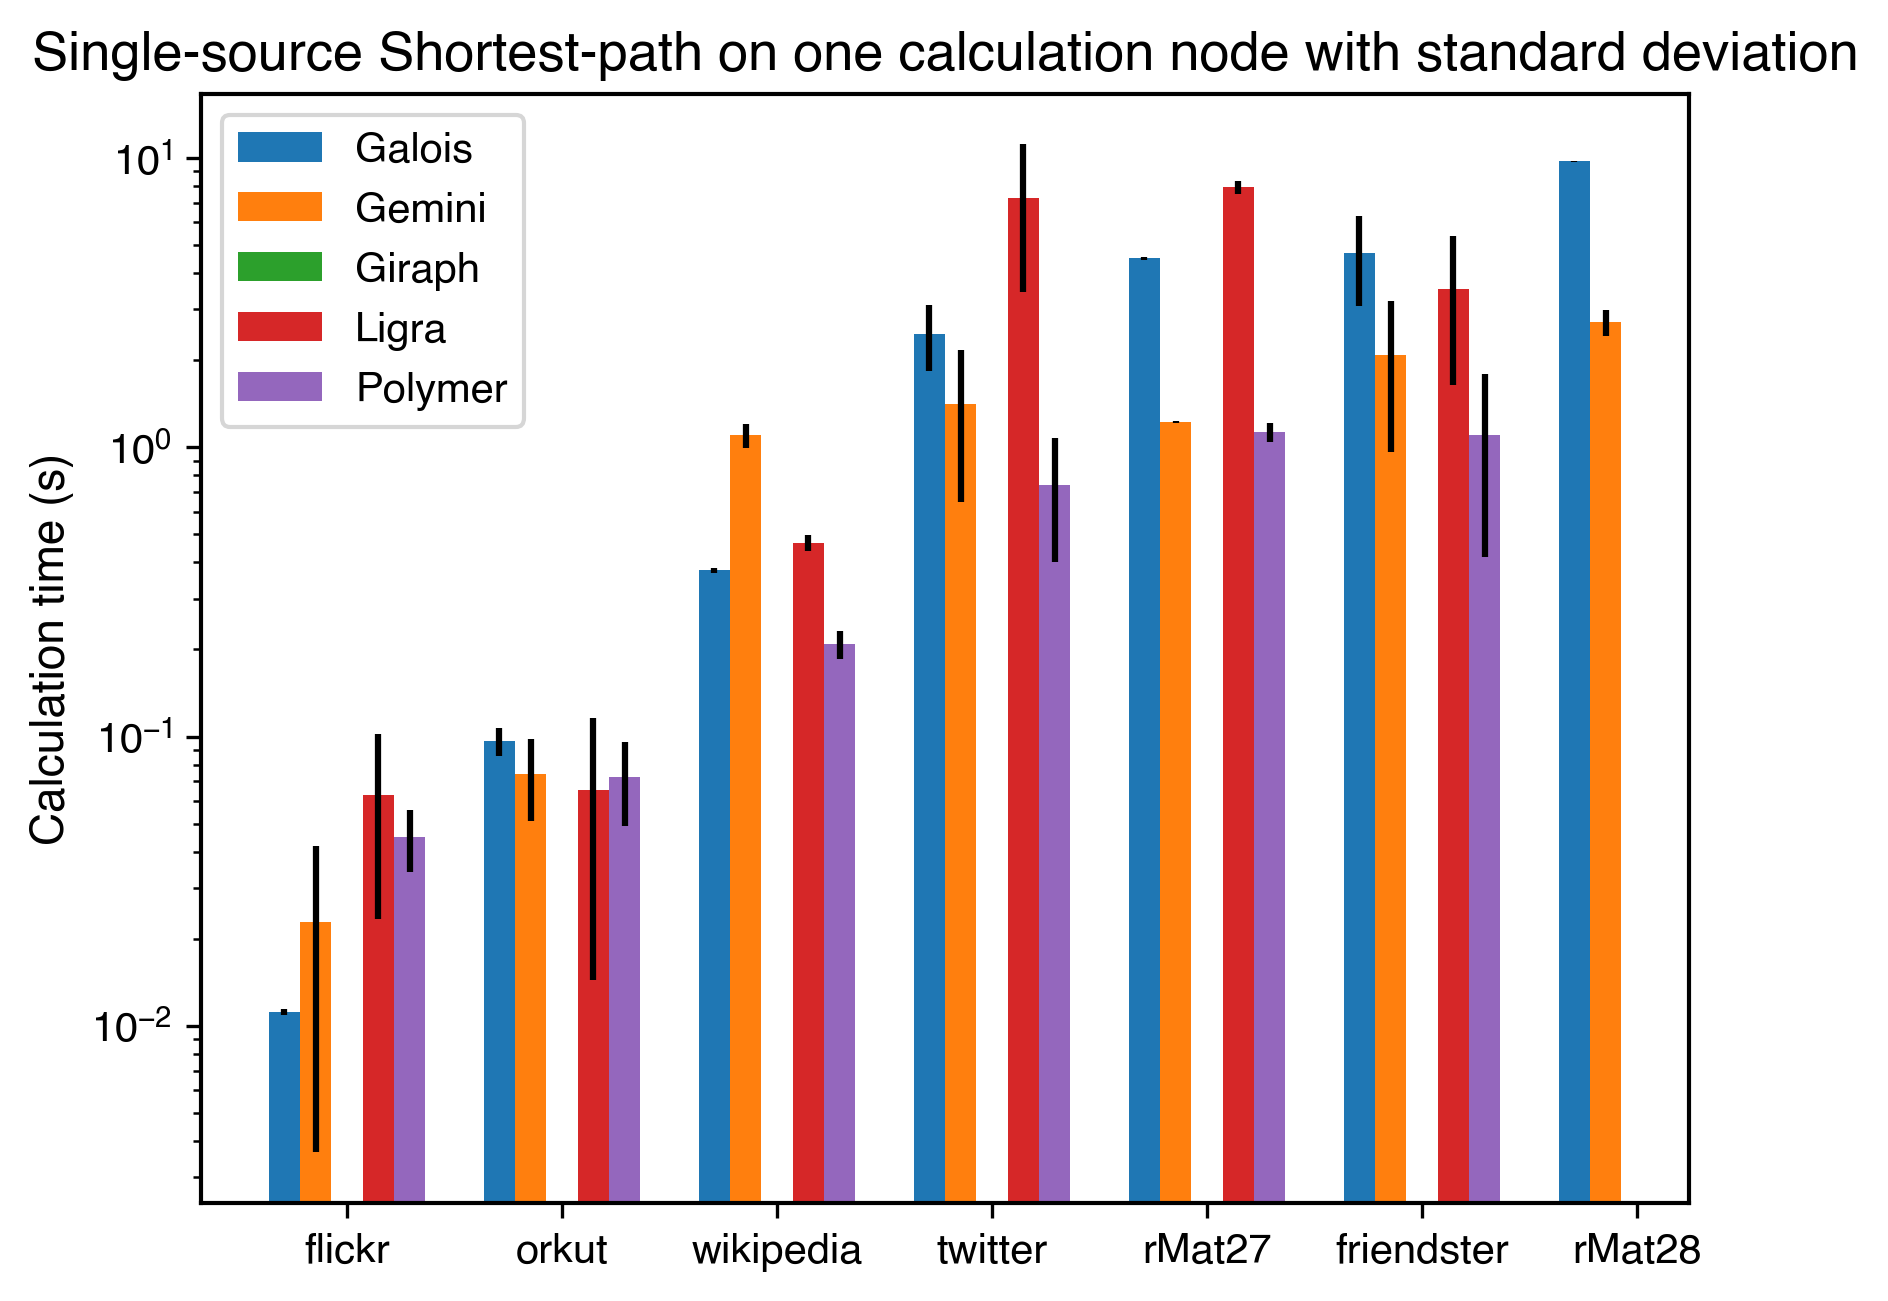
\includegraphics[width=\linewidth]{../../plots/singleNodeSSSP_calcTime.png}
		\caption{Calculation times for SSSP on a single node}
		\label{fig:singleNodeSSSP_calc}
	\end{subfigure}
	\hfil
	\begin{subfigure}{0.3\textwidth}
		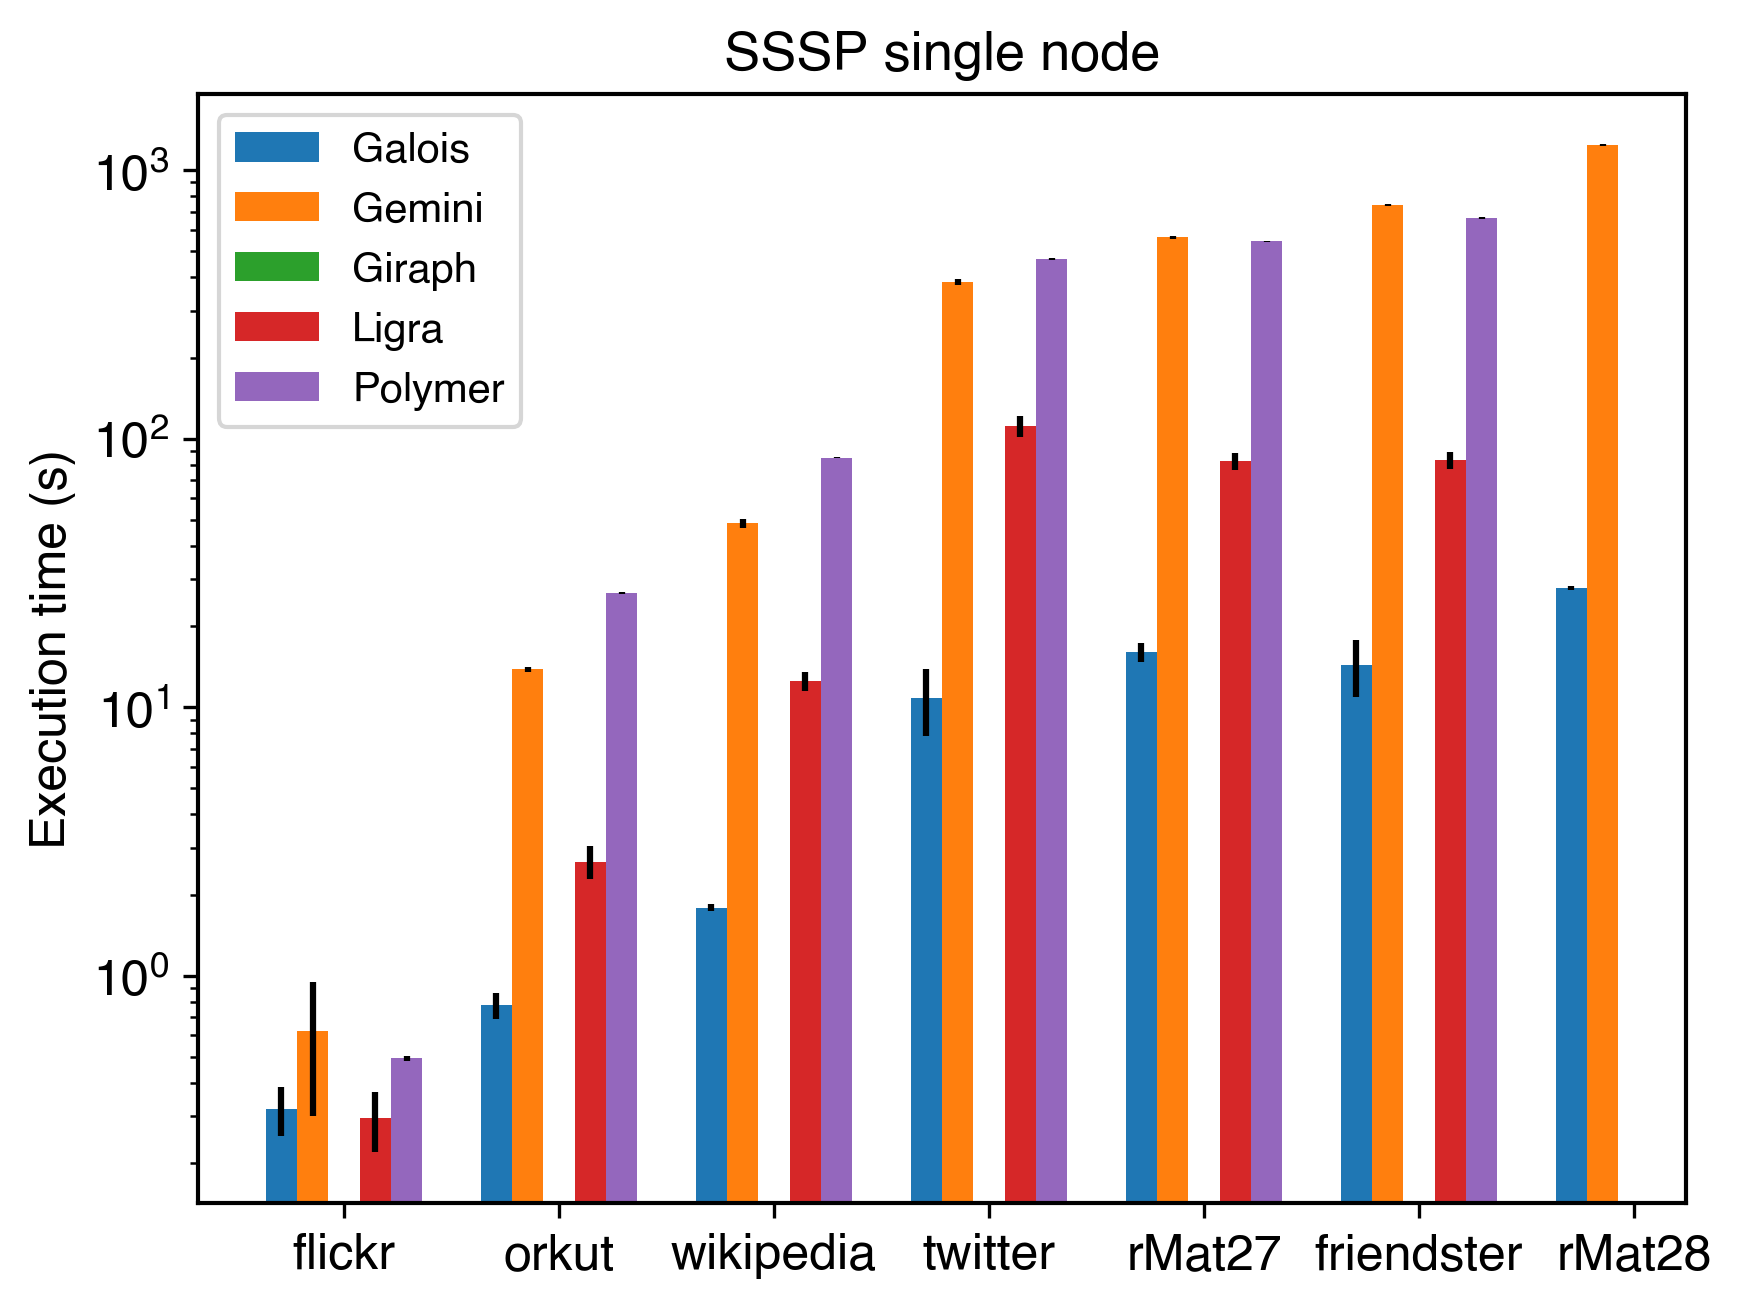
\includegraphics[width=\linewidth]{../../plots/singleNodeSSSP_execTime.png}
		\caption{Execution times for SSSP on a single node}
		\label{fig:singleNodeSSSP_exec}
	\end{subfigure}
	\hfil
	\begin{subfigure}{0.3\textwidth}
		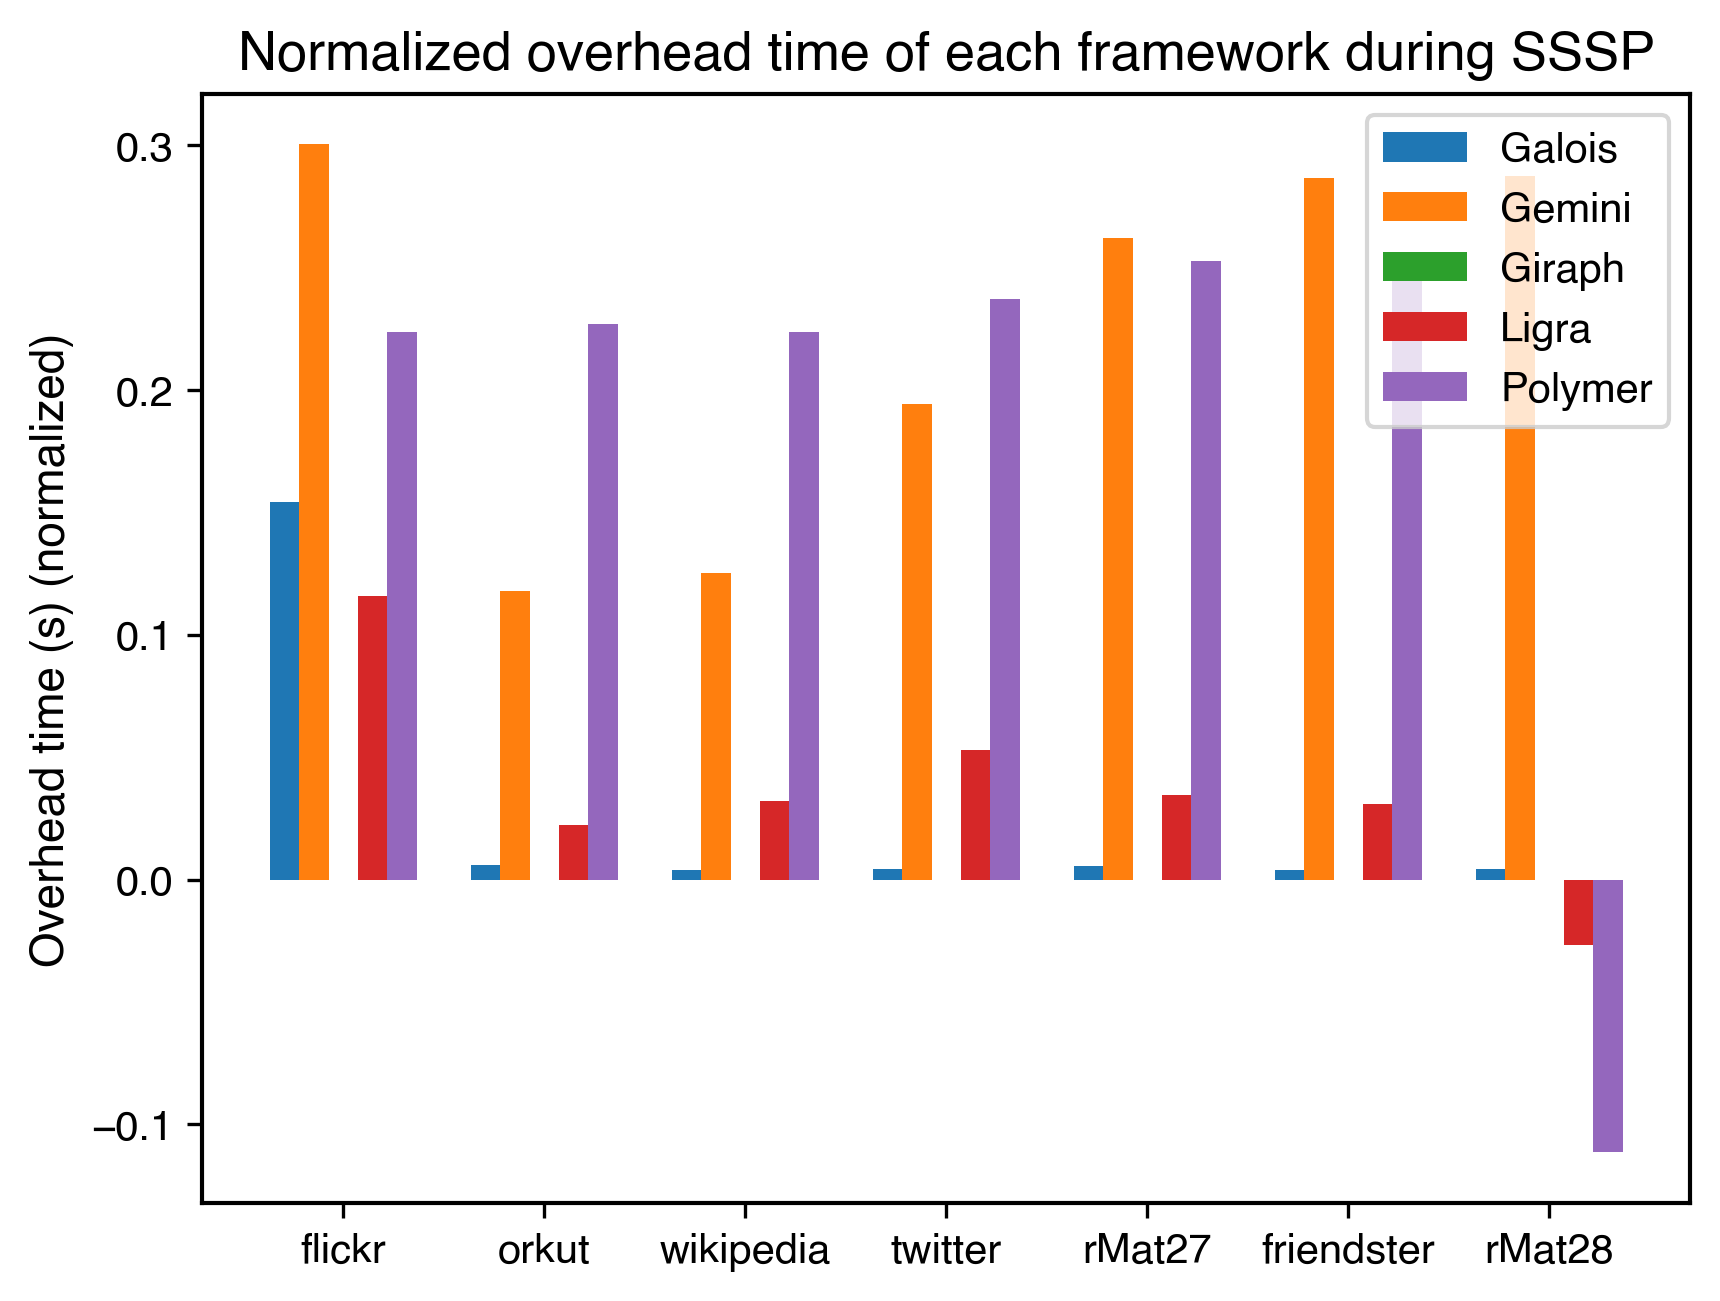
\includegraphics[width=\linewidth]{../../plots/singleNodeSSSP_overheadTimeNormalized.png}
		\caption{Overhead time normalized by the graph size in million edges}
		\label{fig:singleNodeSSSP_overheadNormalized}
	\end{subfigure}
	\caption{Average times on a single computation node, black bars represent one standard deviation in our testing.}
	\label{fig:singleNodeSSSP}
\end{figure*}




\begin{figure*}[t!]
	\begin{subfigure}{0.3\textwidth}
		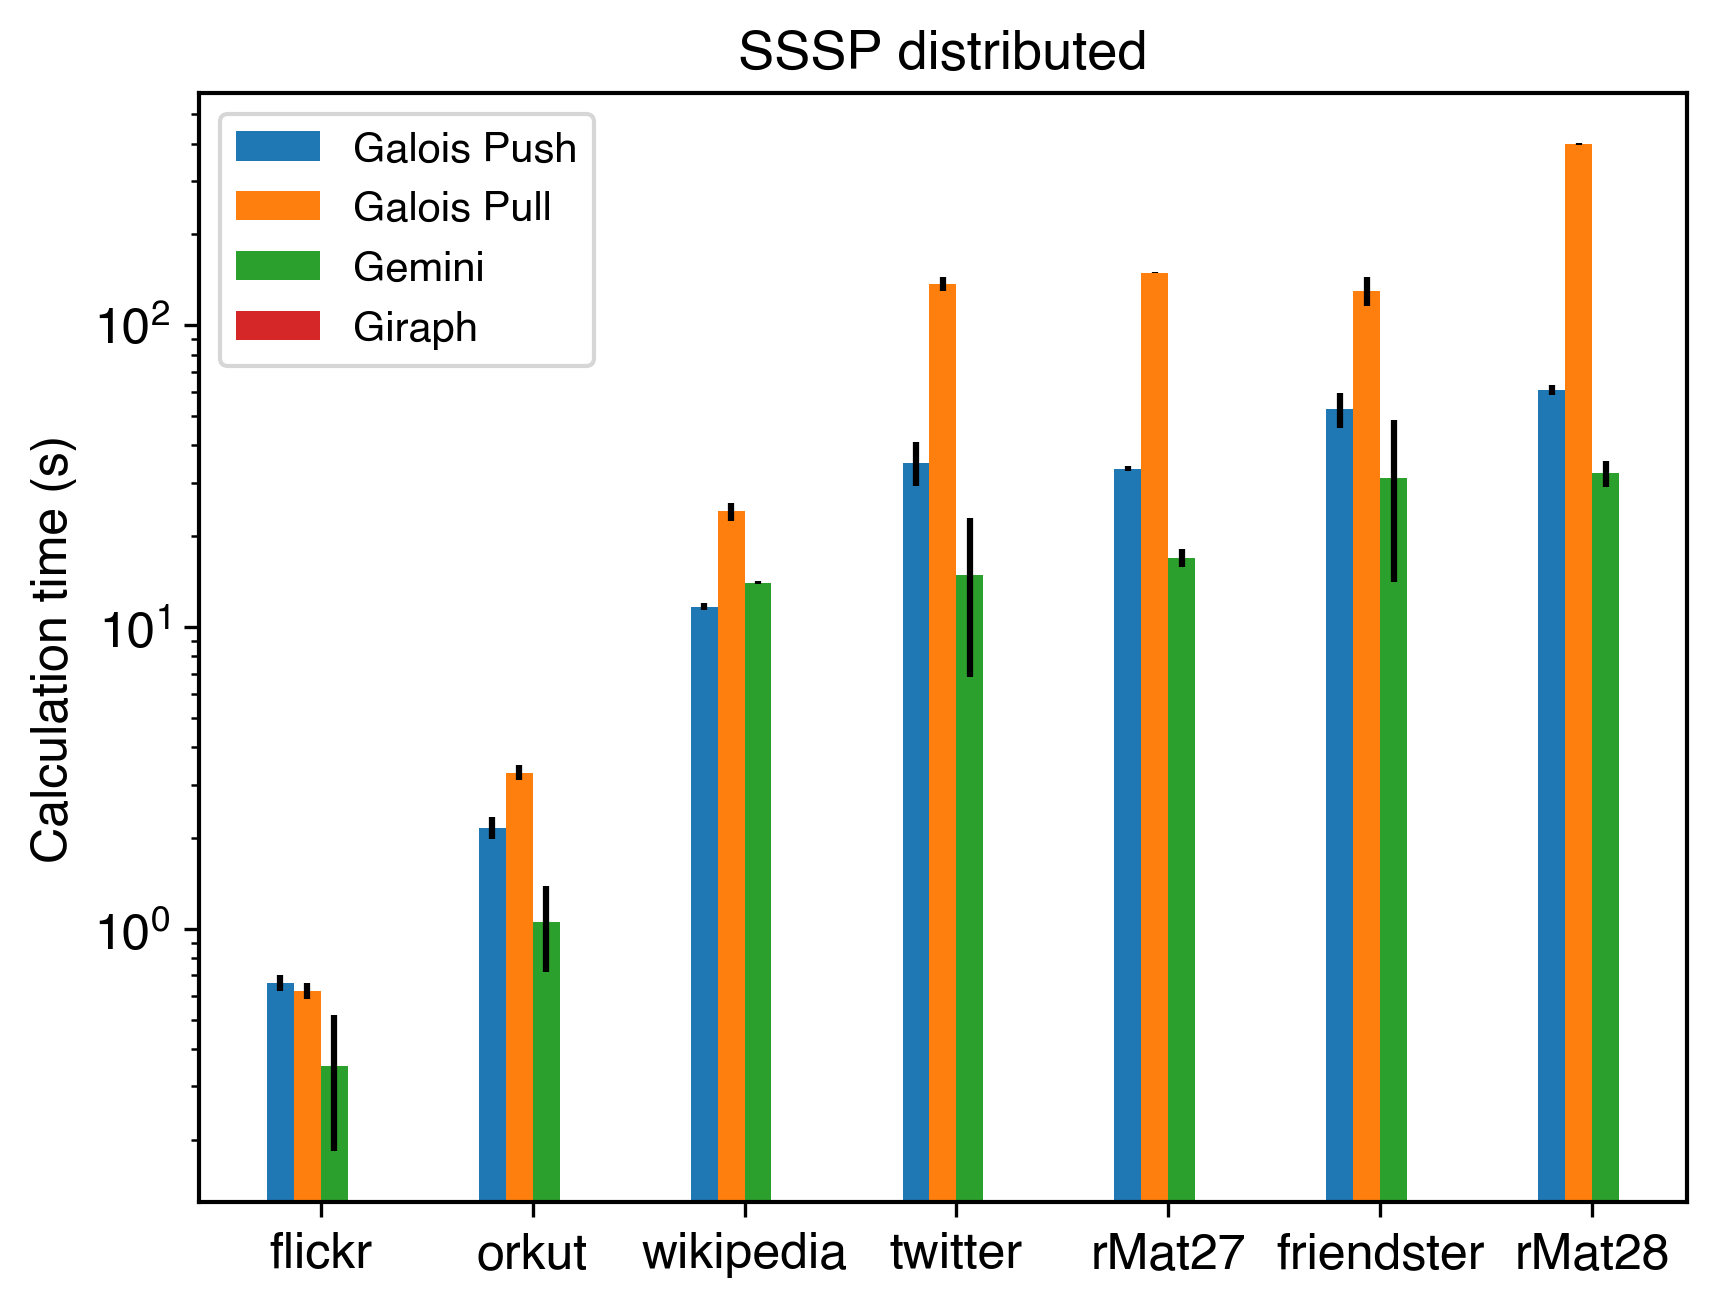
\includegraphics[width=\linewidth]{../../plots/distributedSSSP_calcTime.png}
		\caption{Calculation times for distributed SSSP}
		\label{fig:distributedSSSP_calc}
	\end{subfigure}
	\hfil
	\begin{subfigure}{0.3\textwidth}
		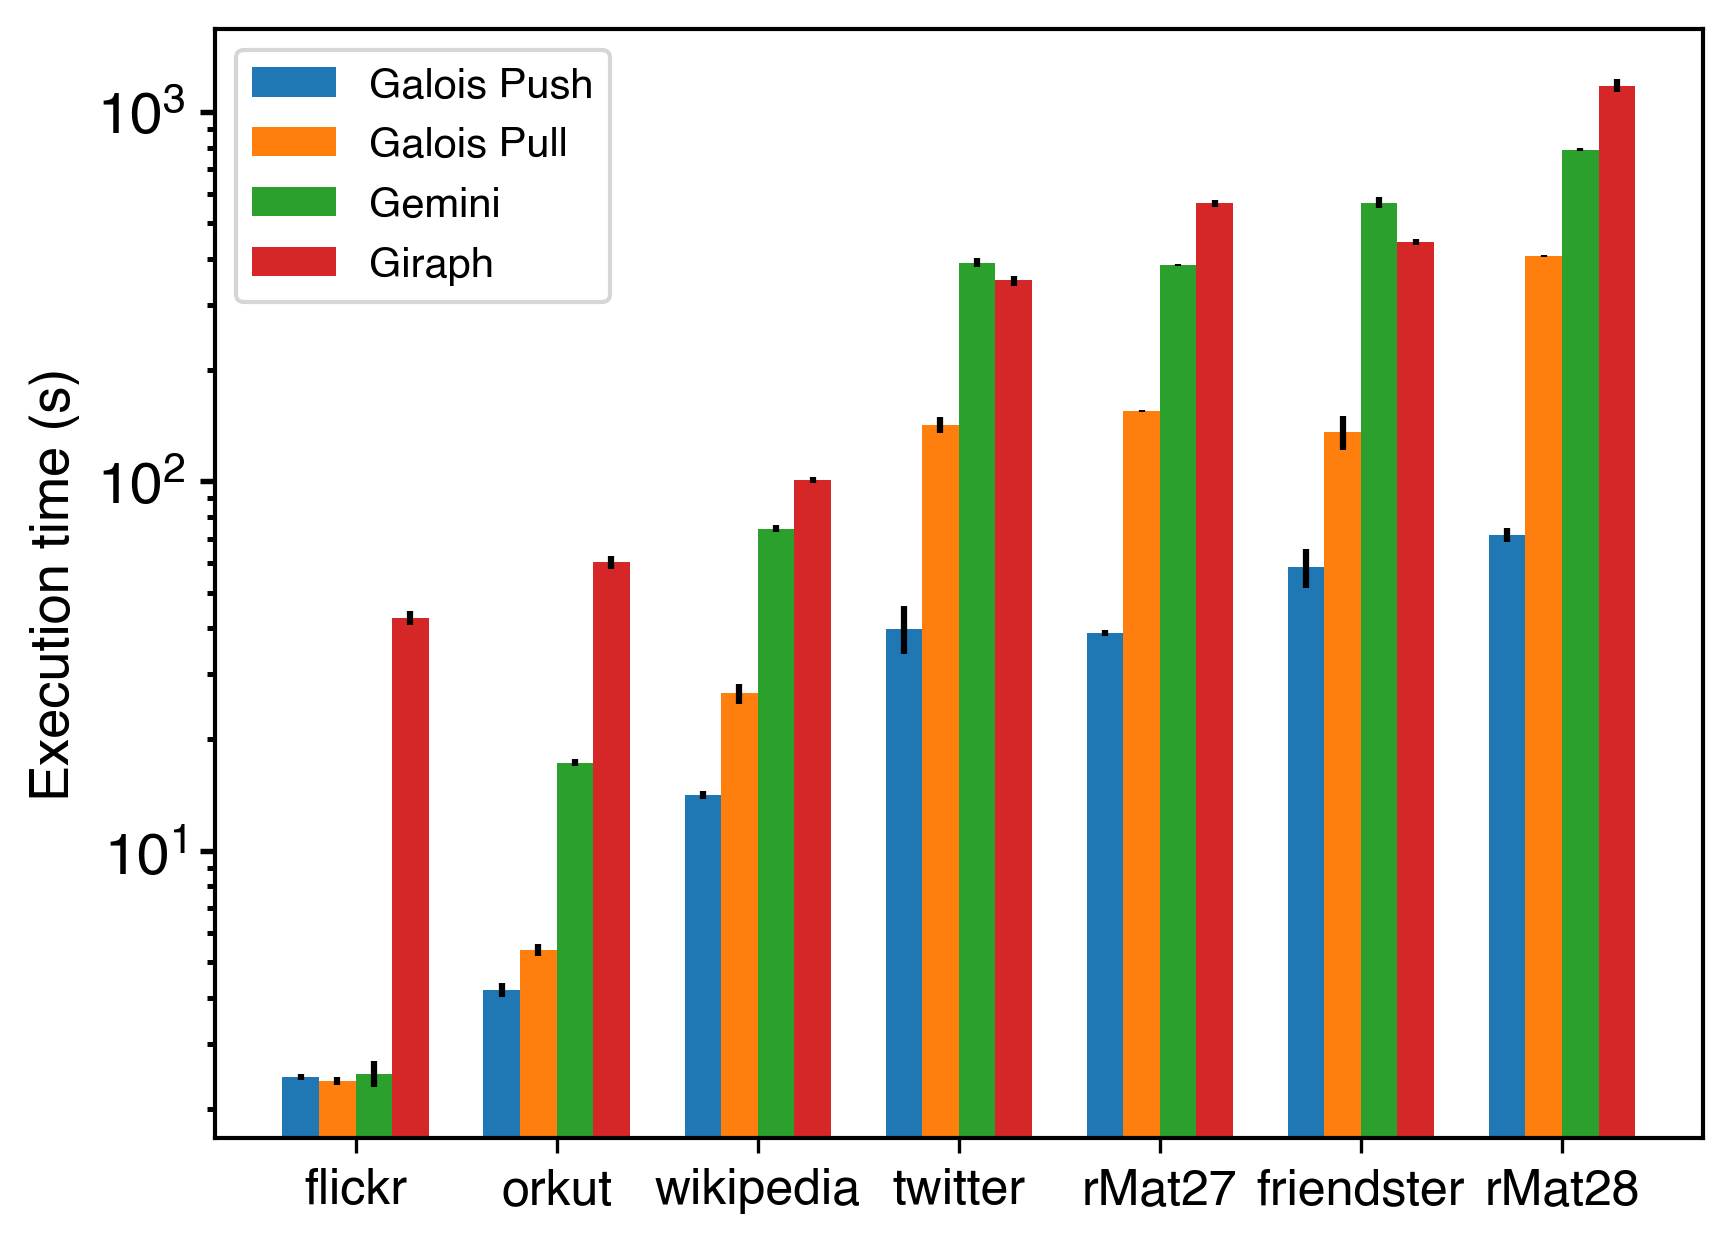
\includegraphics[width=\linewidth]{../../plots/distributedSSSP_execTime.png}
		\caption{Execution times for distributed SSSP}
		\label{fig:distributedSSSP_exec}
	\end{subfigure}
	\hfil
	\begin{subfigure}{0.3\textwidth}
		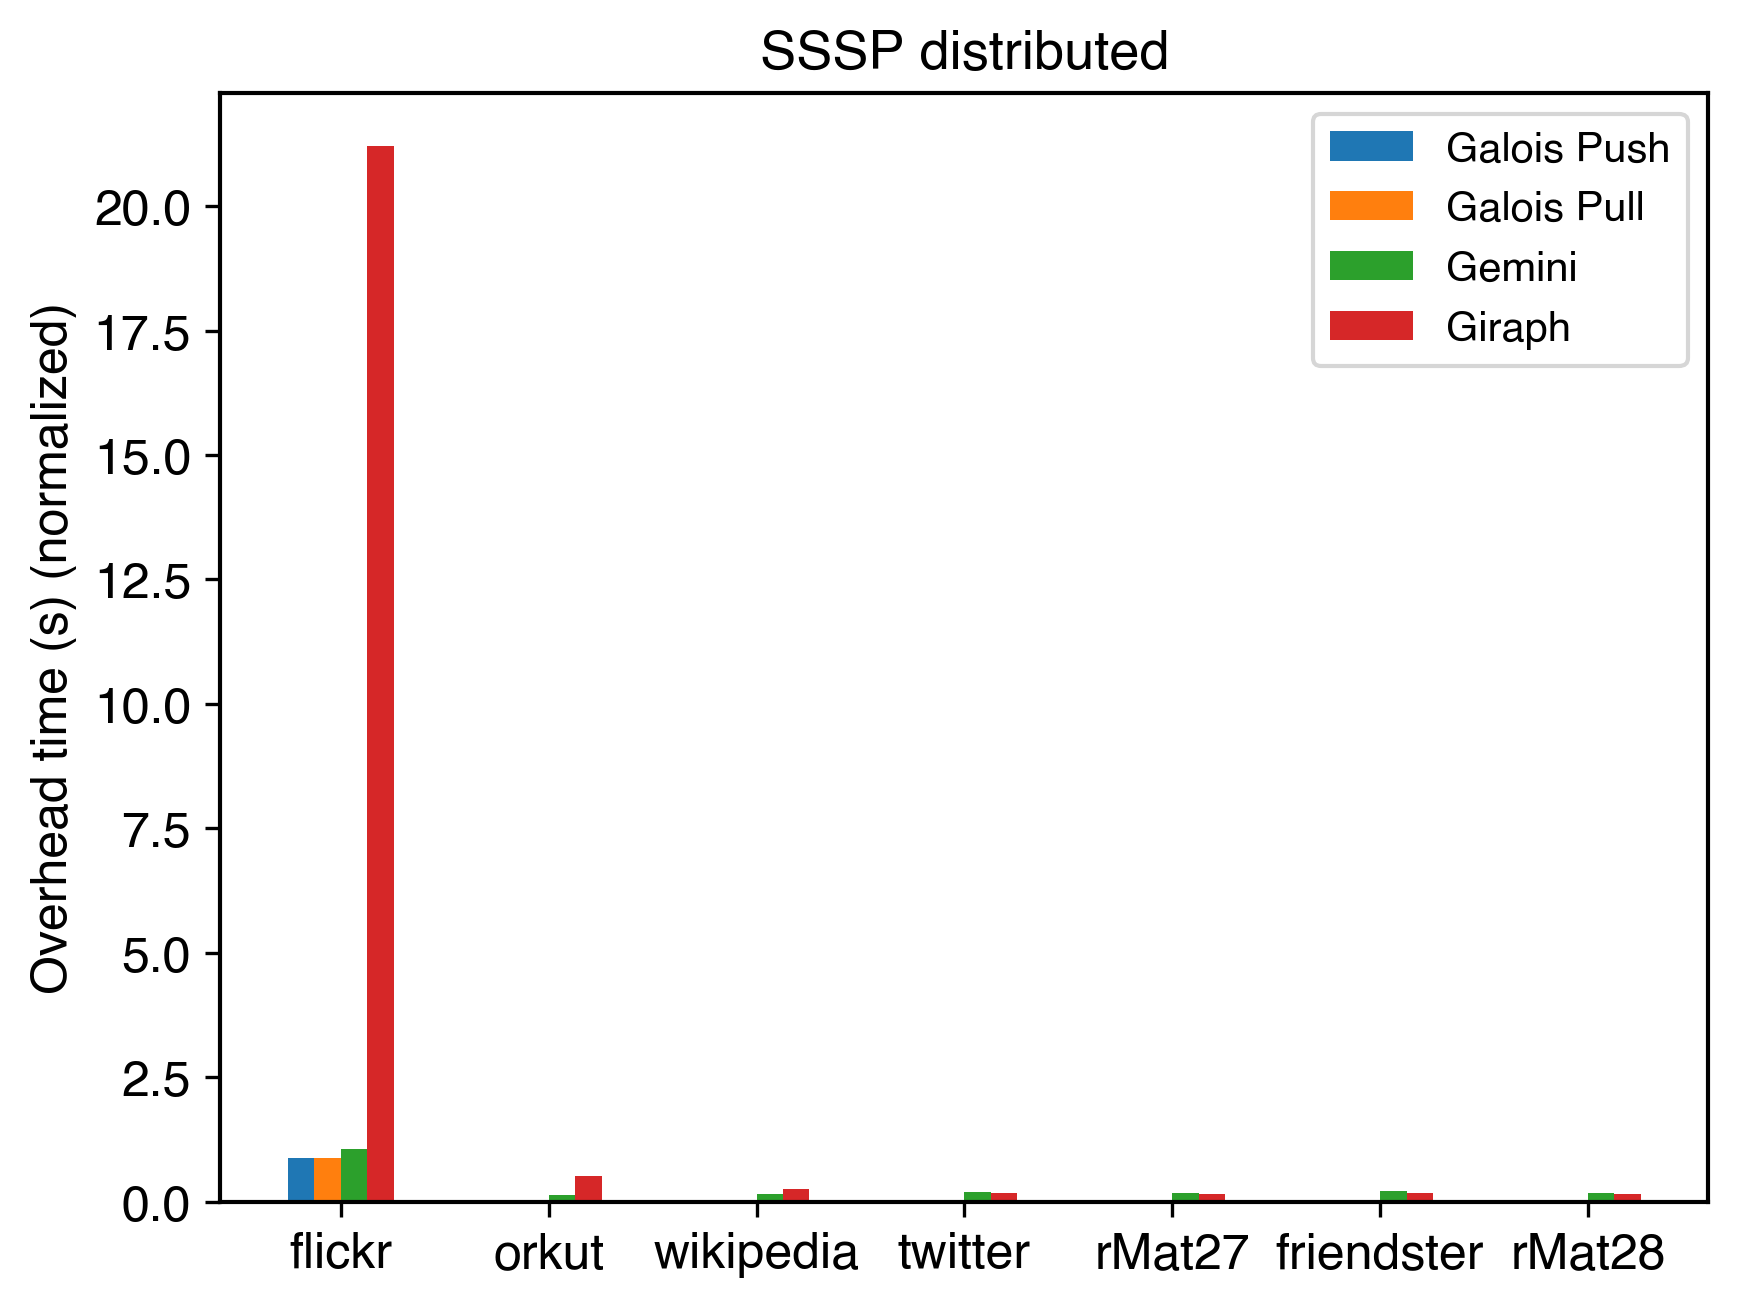
\includegraphics[width=\linewidth]{../../plots/distributedSSSP_overheadTimeNormalized.png}
		\caption{Overhead time normalized by the graph size in million edges}
		\label{fig:distributedSSSP_overheadNormalized}
	\end{subfigure}
	\caption{Average times on the distributed cluster, black bars represent one standard deviation in our testing.}
	\label{fig:distributedSSSP}
\end{figure*}




\subsection{Breadth-first search}
In these figures, Galois with 96 threads is shown. Again, we show the impact of Galois' thread count in \autoref{sec:galois_speedup}.
\begin{figure*}
	\begin{subfigure}{0.3\textwidth}
		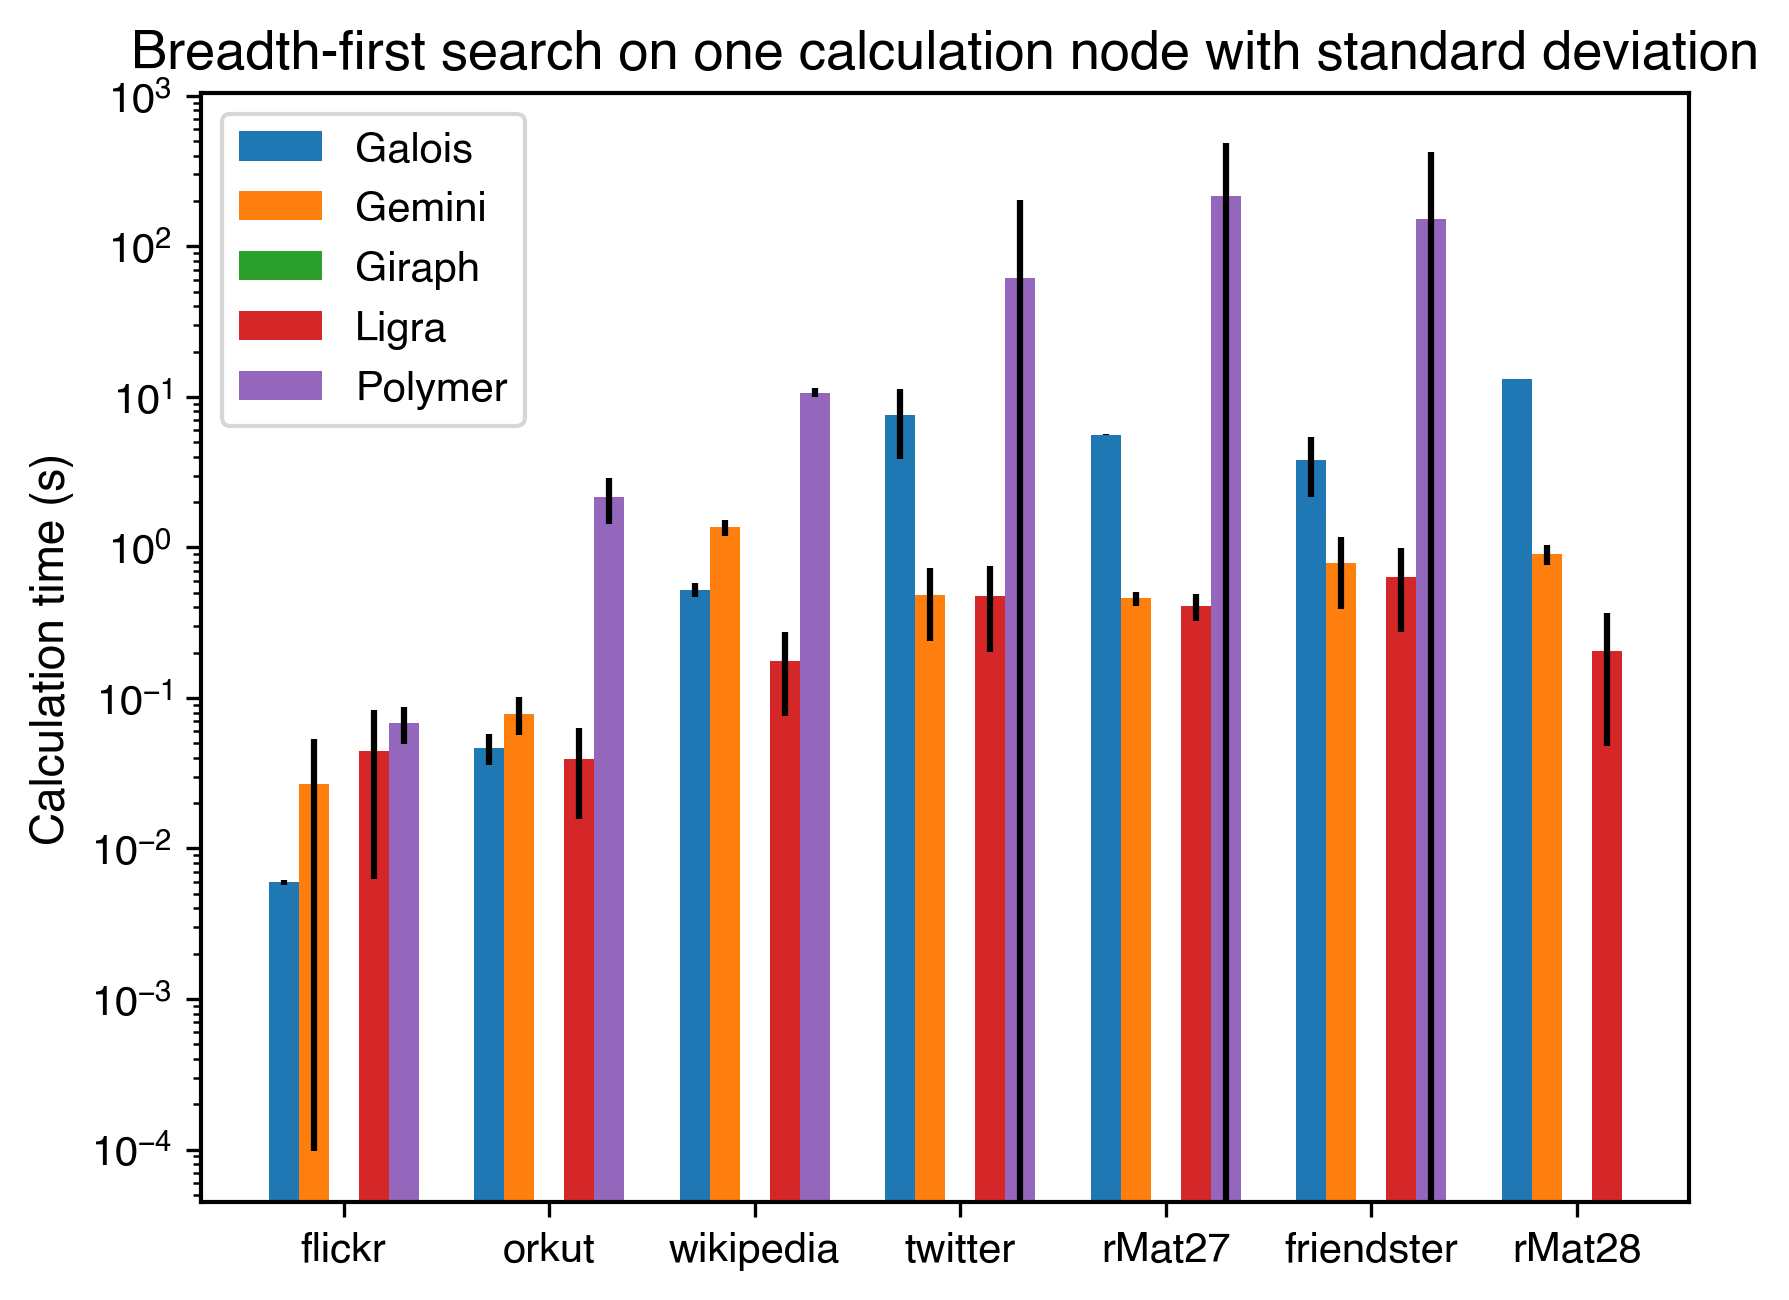
\includegraphics[width=\linewidth]{../../plots/singleNodeBFS_calcTime.png}
		\caption{Calculation times for BFS on a single node}
		\label{fig:singleNodeBFS_calc}
	\end{subfigure}
	\hfil
	\begin{subfigure}{0.3\textwidth}
		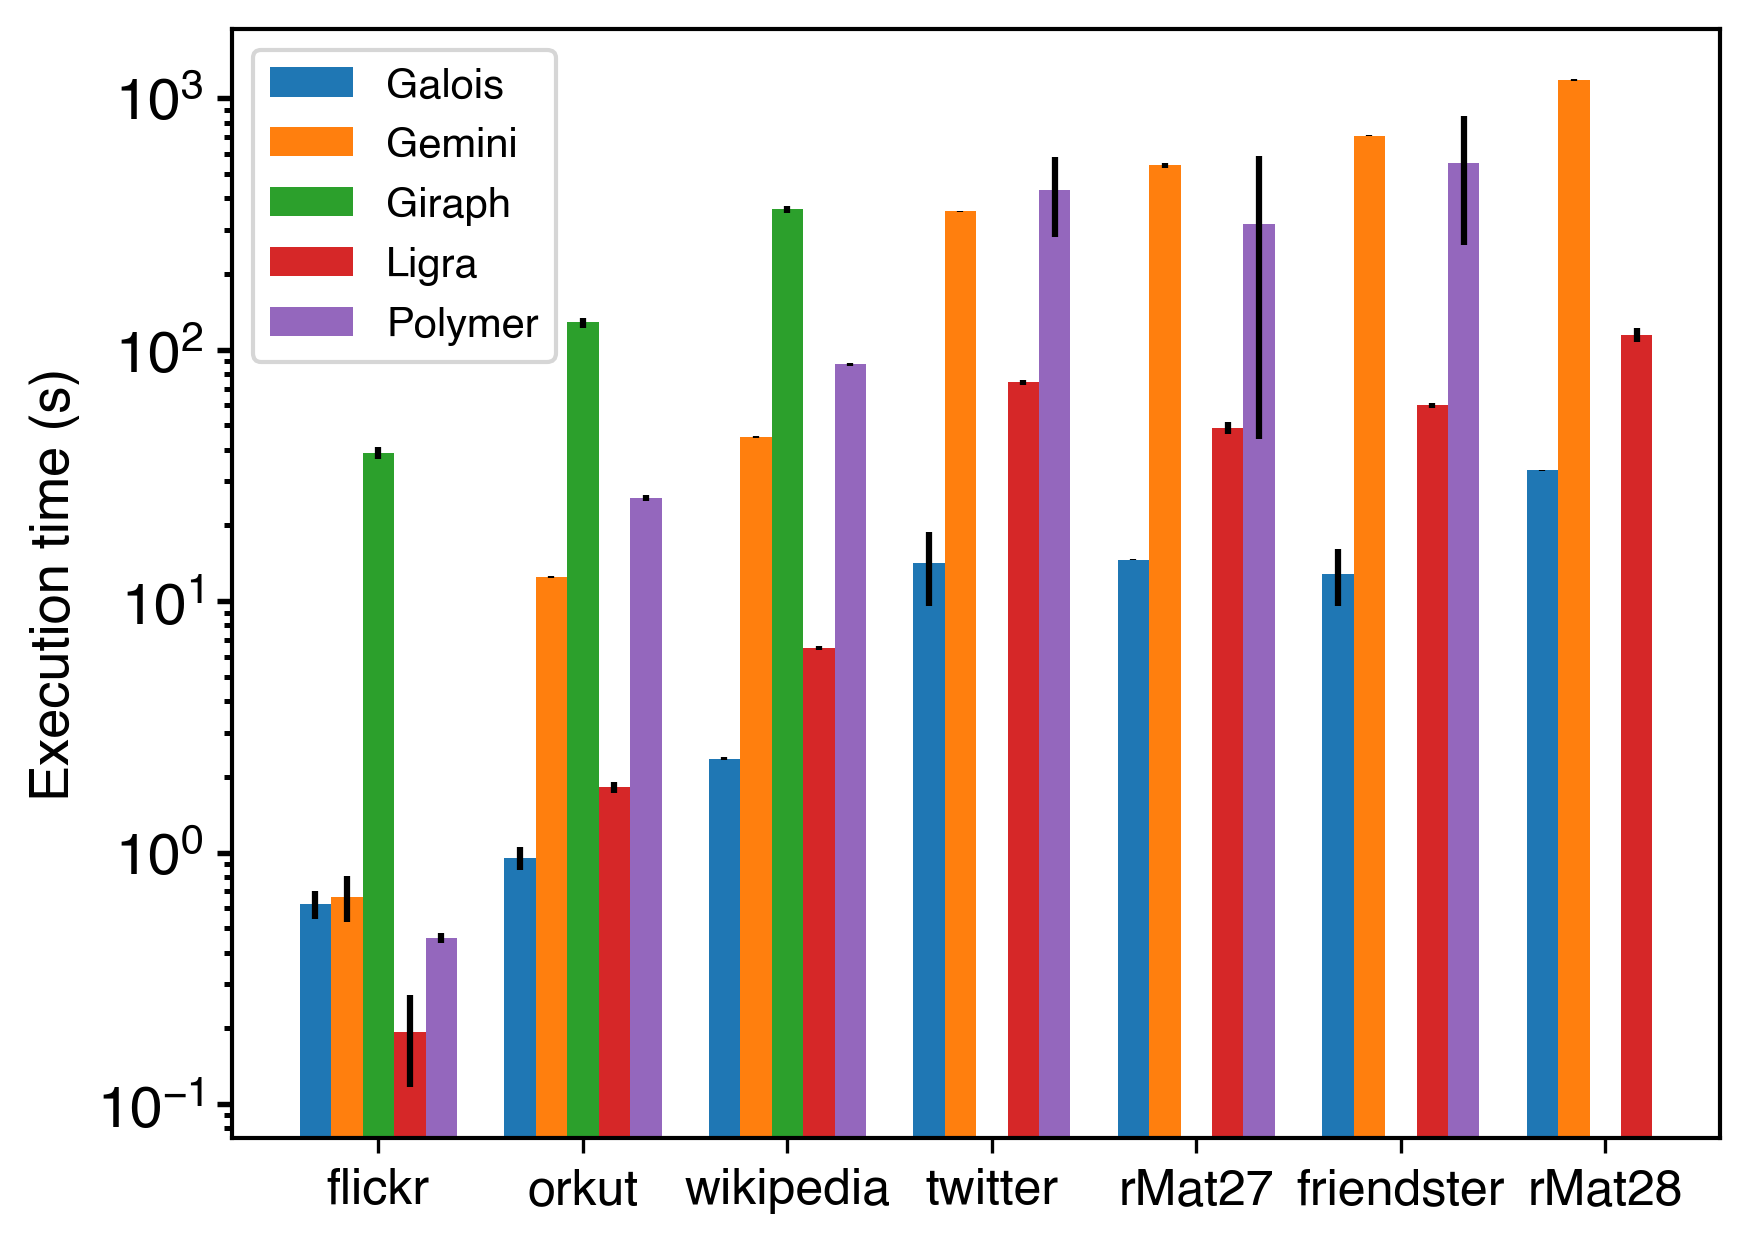
\includegraphics[width=\linewidth]{../../plots/singleNodeBFS_execTime.png}
		\caption{Execution times for BFS on a single node}
		\label{fig:singleNodeBFS_exec}
	\end{subfigure}
	\hfil
	\begin{subfigure}{0.3\textwidth}
		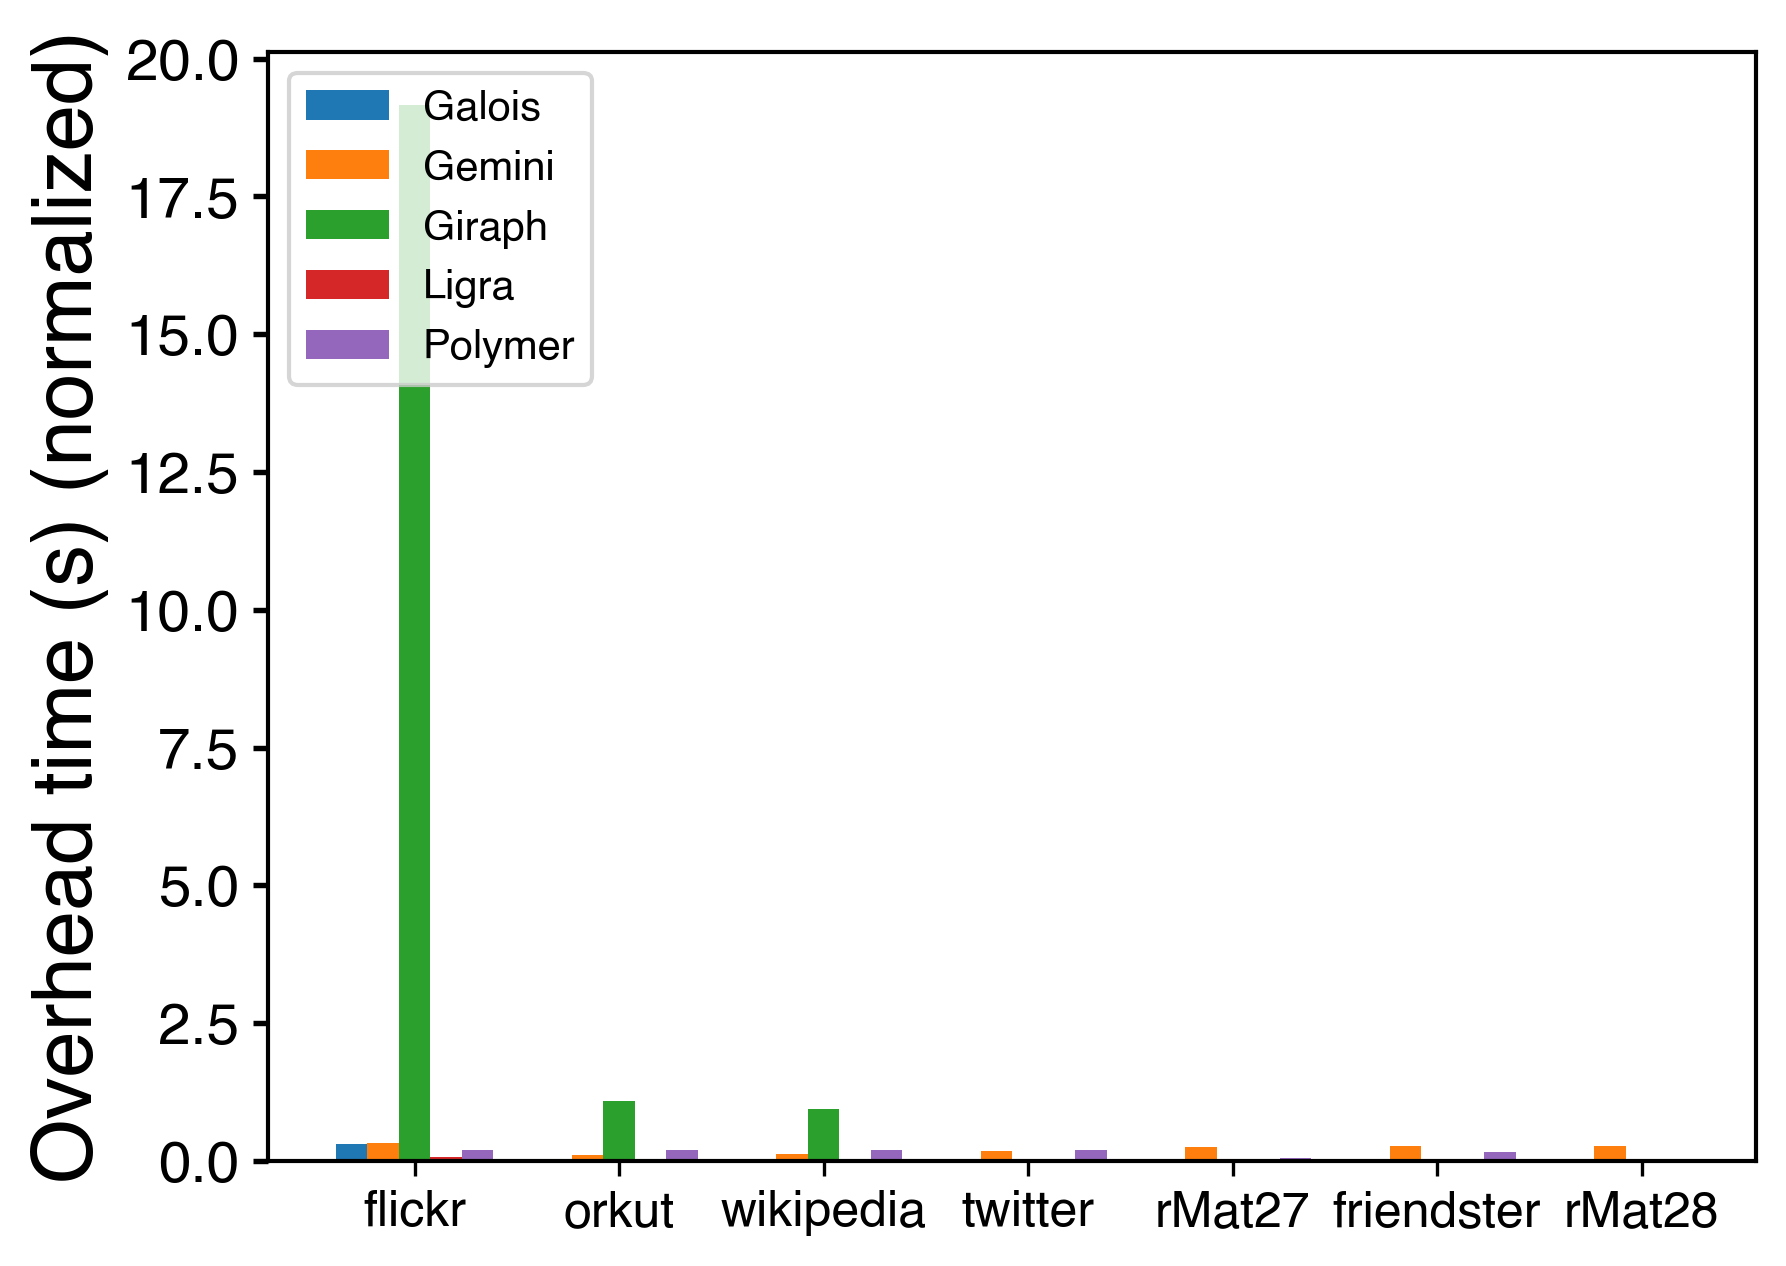
\includegraphics[width=\linewidth]{../../plots/singleNodeBFS_overheadTimeNormalized.png}
		\caption{Overhead time normalized by the graph size in million edges}
		\label{fig:singleNodeBFS_overheadNormalized}
	\end{subfigure}
	
	\caption{Average times on a single computation node, black bars represent one standard deviation in our testing}
\end{figure*}




\begin{figure*}
	\begin{subfigure}{0.3\textwidth}
		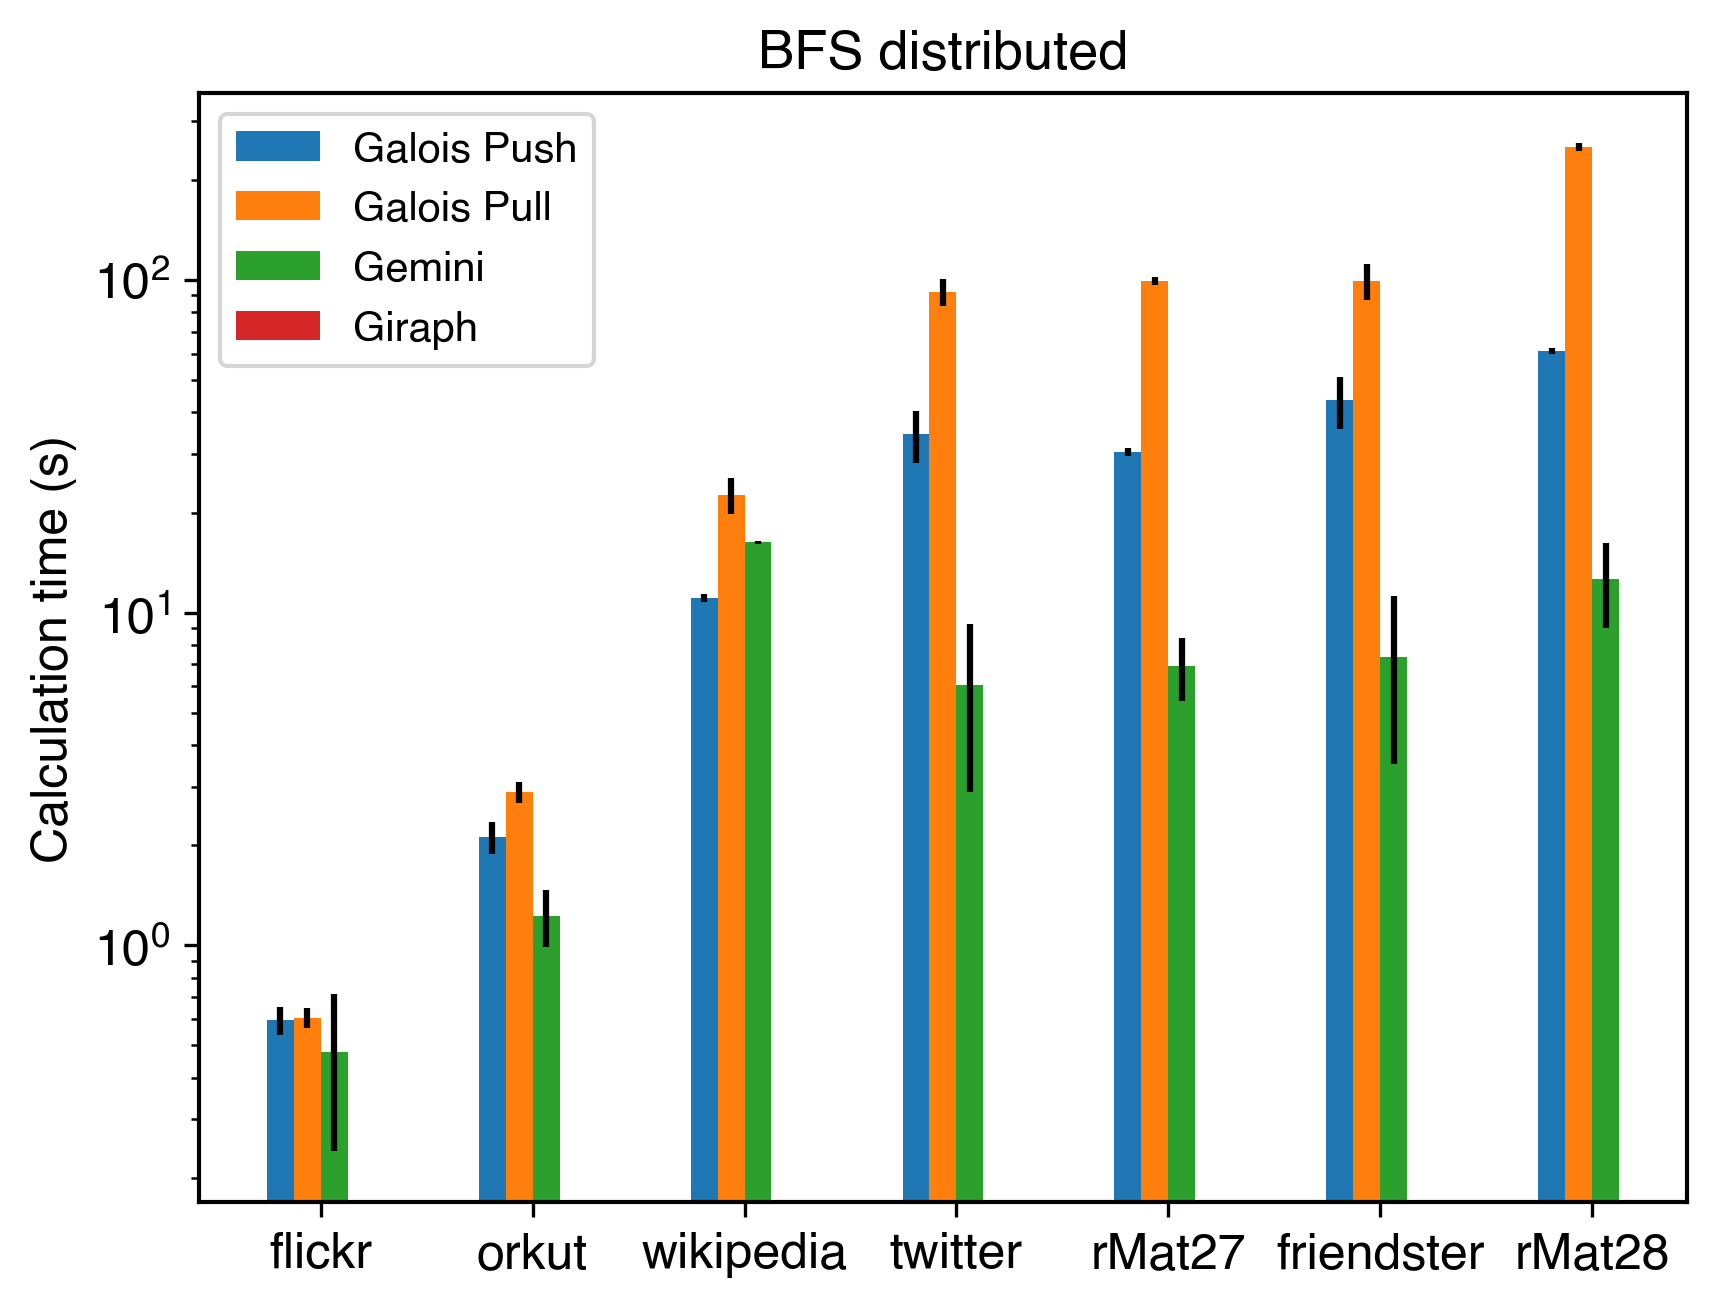
\includegraphics[width=\linewidth]{../../plots/distributedBFS_calcTime.png}
		\caption{Calculation times for distributed BFS}
		\label{fig:distributedBFS_calc}
	\end{subfigure}
	\hfil
	\begin{subfigure}{0.3\textwidth}
		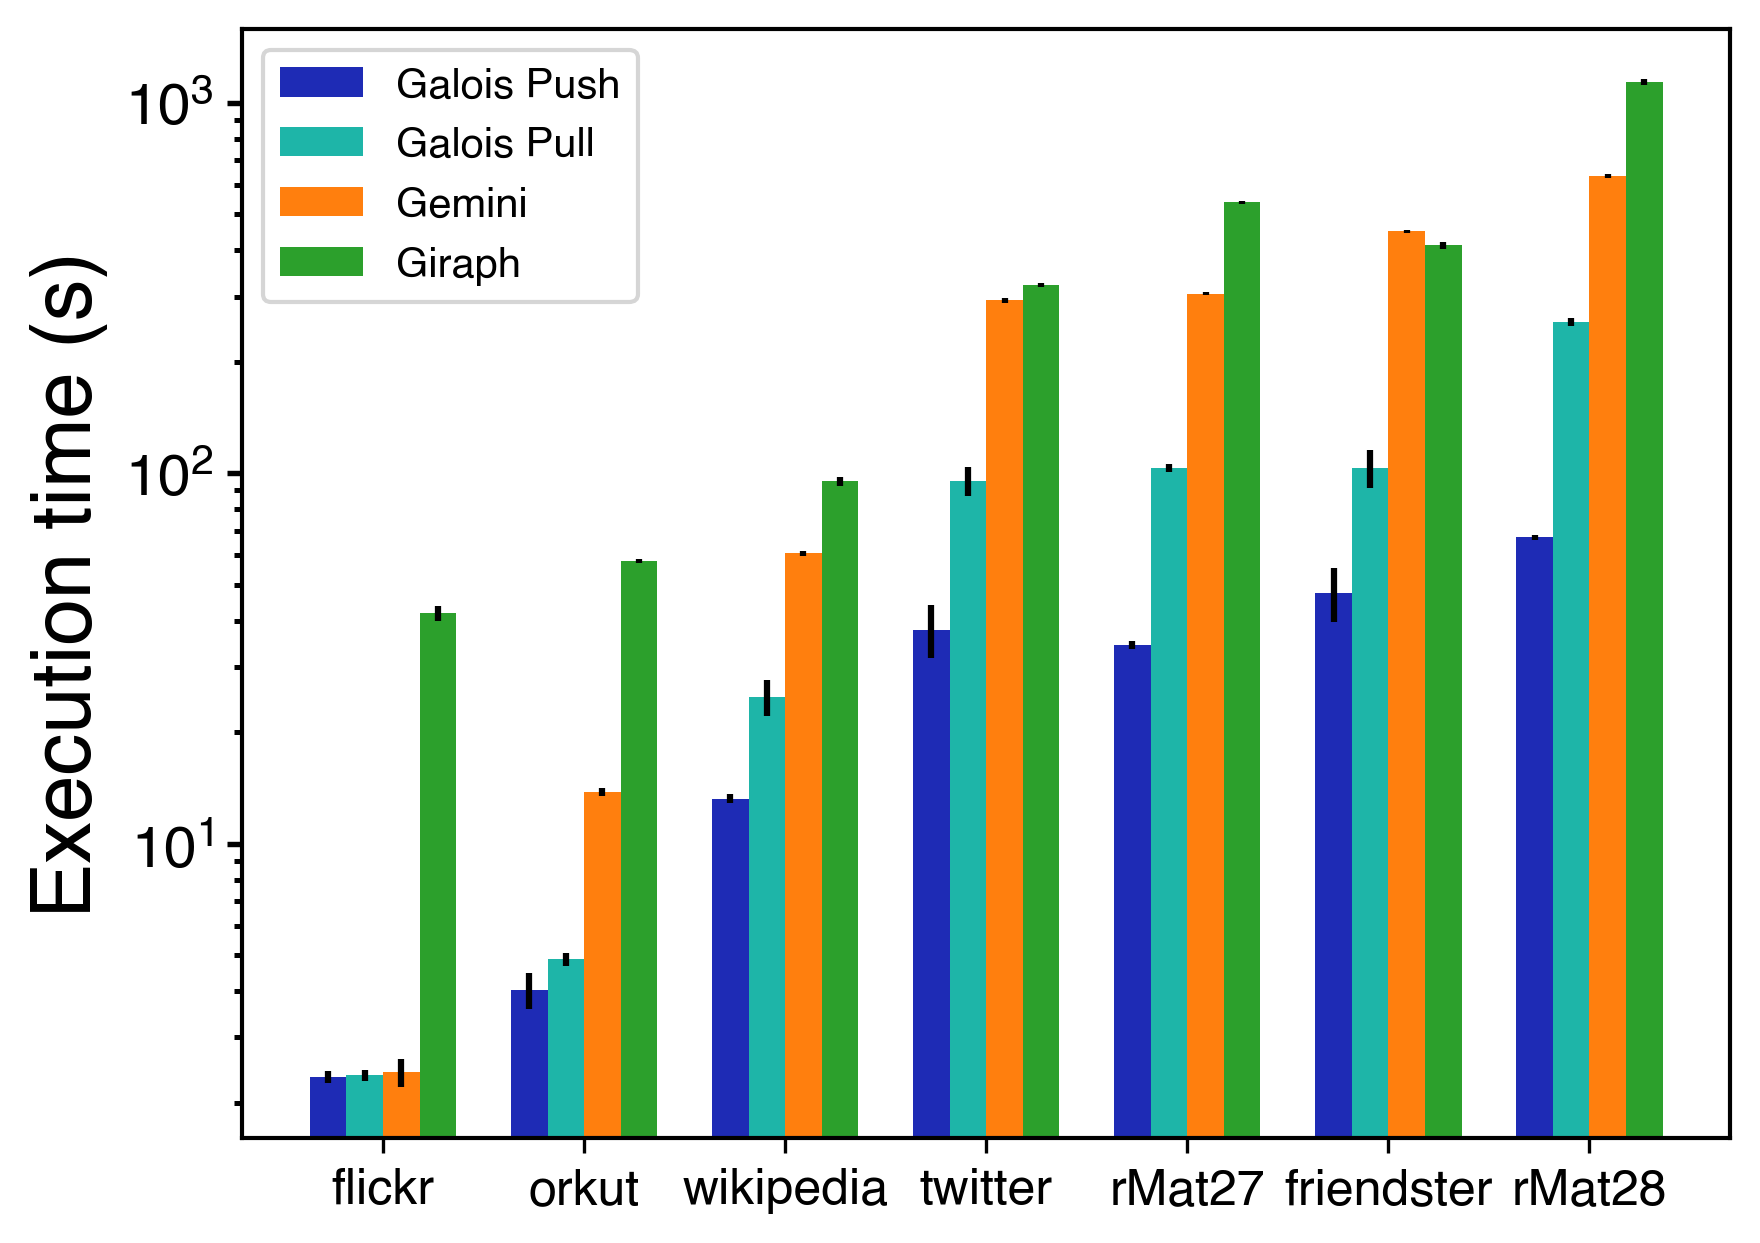
\includegraphics[width=\linewidth]{../../plots/distributedBFS_execTime.png}
		\caption{Execution times for distributed BFS}
		\label{fig:distributedBFS_exec}
	\end{subfigure}
	\hfil
	\begin{subfigure}{0.3\textwidth}
		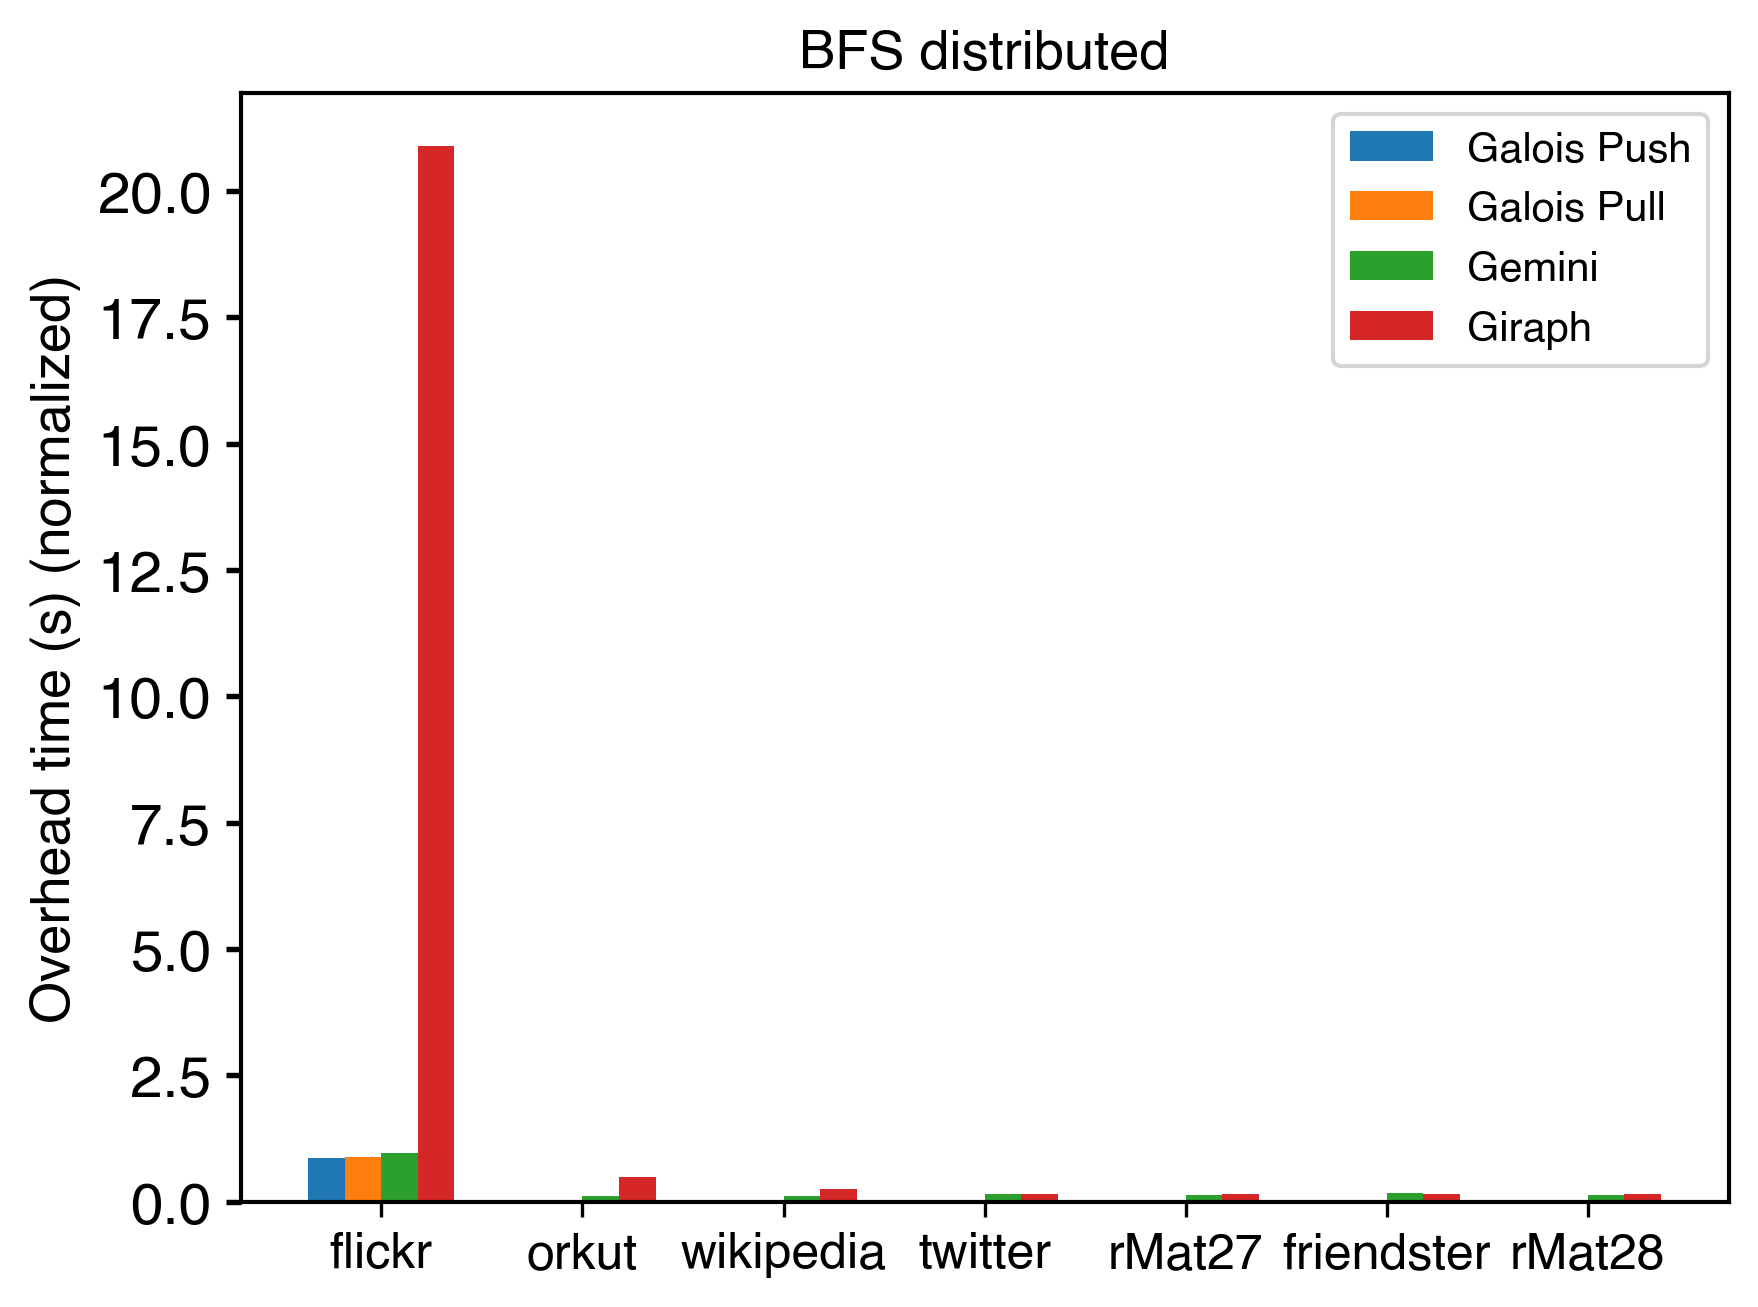
\includegraphics[width=\linewidth]{../../plots/distributedBFS_overheadTimeNormalized.png}
		\caption{Overhead time normalized by the graph size in million edges}
		\label{fig:distributedBFS_overheadNormalized}
	\end{subfigure}
	
	\caption{Average times on the distributed cluster, black bars represent one standard deviation in our testing}
\end{figure*}



\subsection{PageRank}
















\subsection{Galois speedup}
\label{sec:galois_speedup}
For Galois we 


\begin{figure}
	\begin{subfigure}{\columnwidth}
		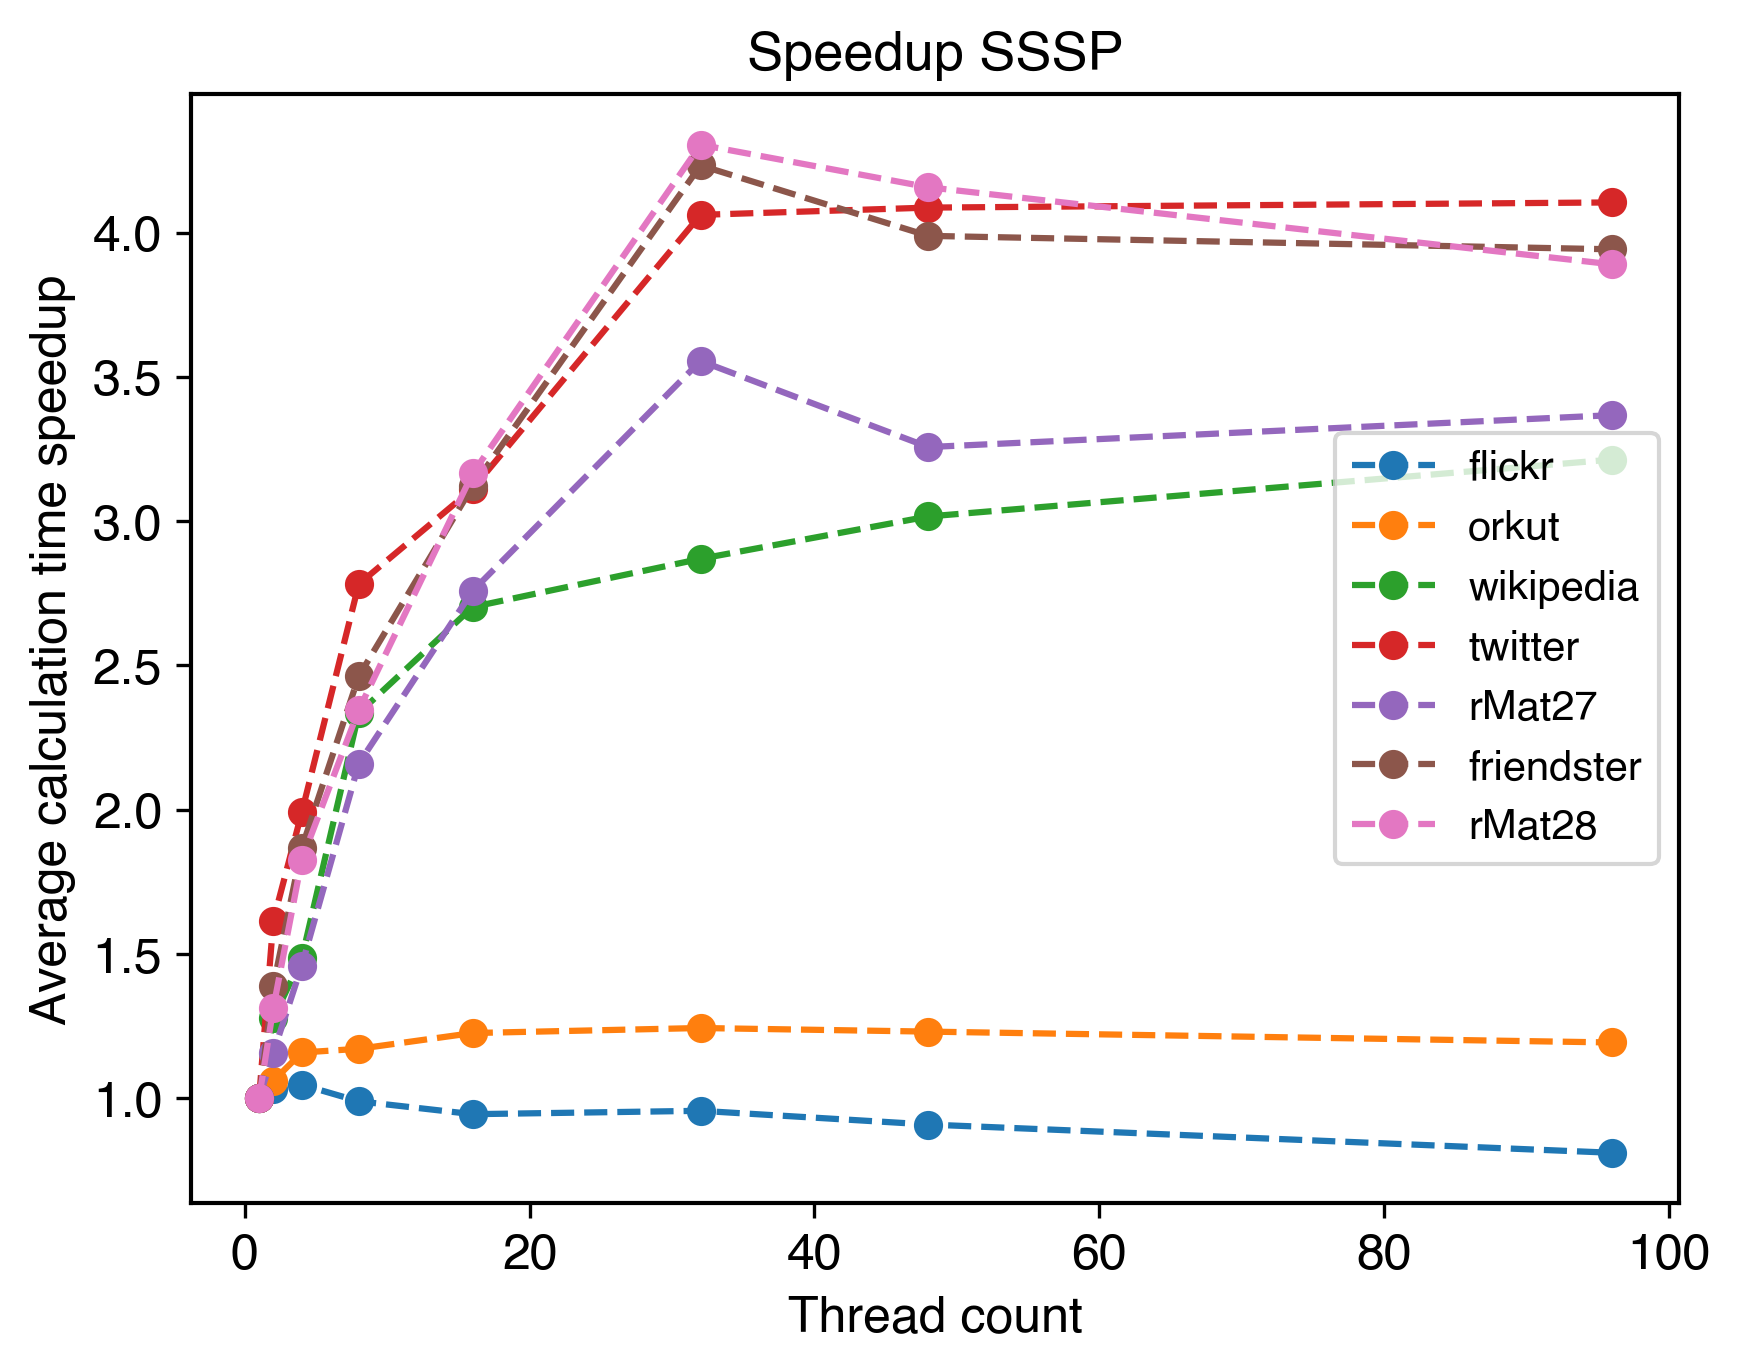
\includegraphics[width=\linewidth]{../../plots/singleNodeSSSPGaloisThreads.png}
		\caption{Single-source Shortest-paths}
		\label{fig:singleNodeSSSPGaloisThreads}
	\end{subfigure}
	\begin{subfigure}{\columnwidth}
		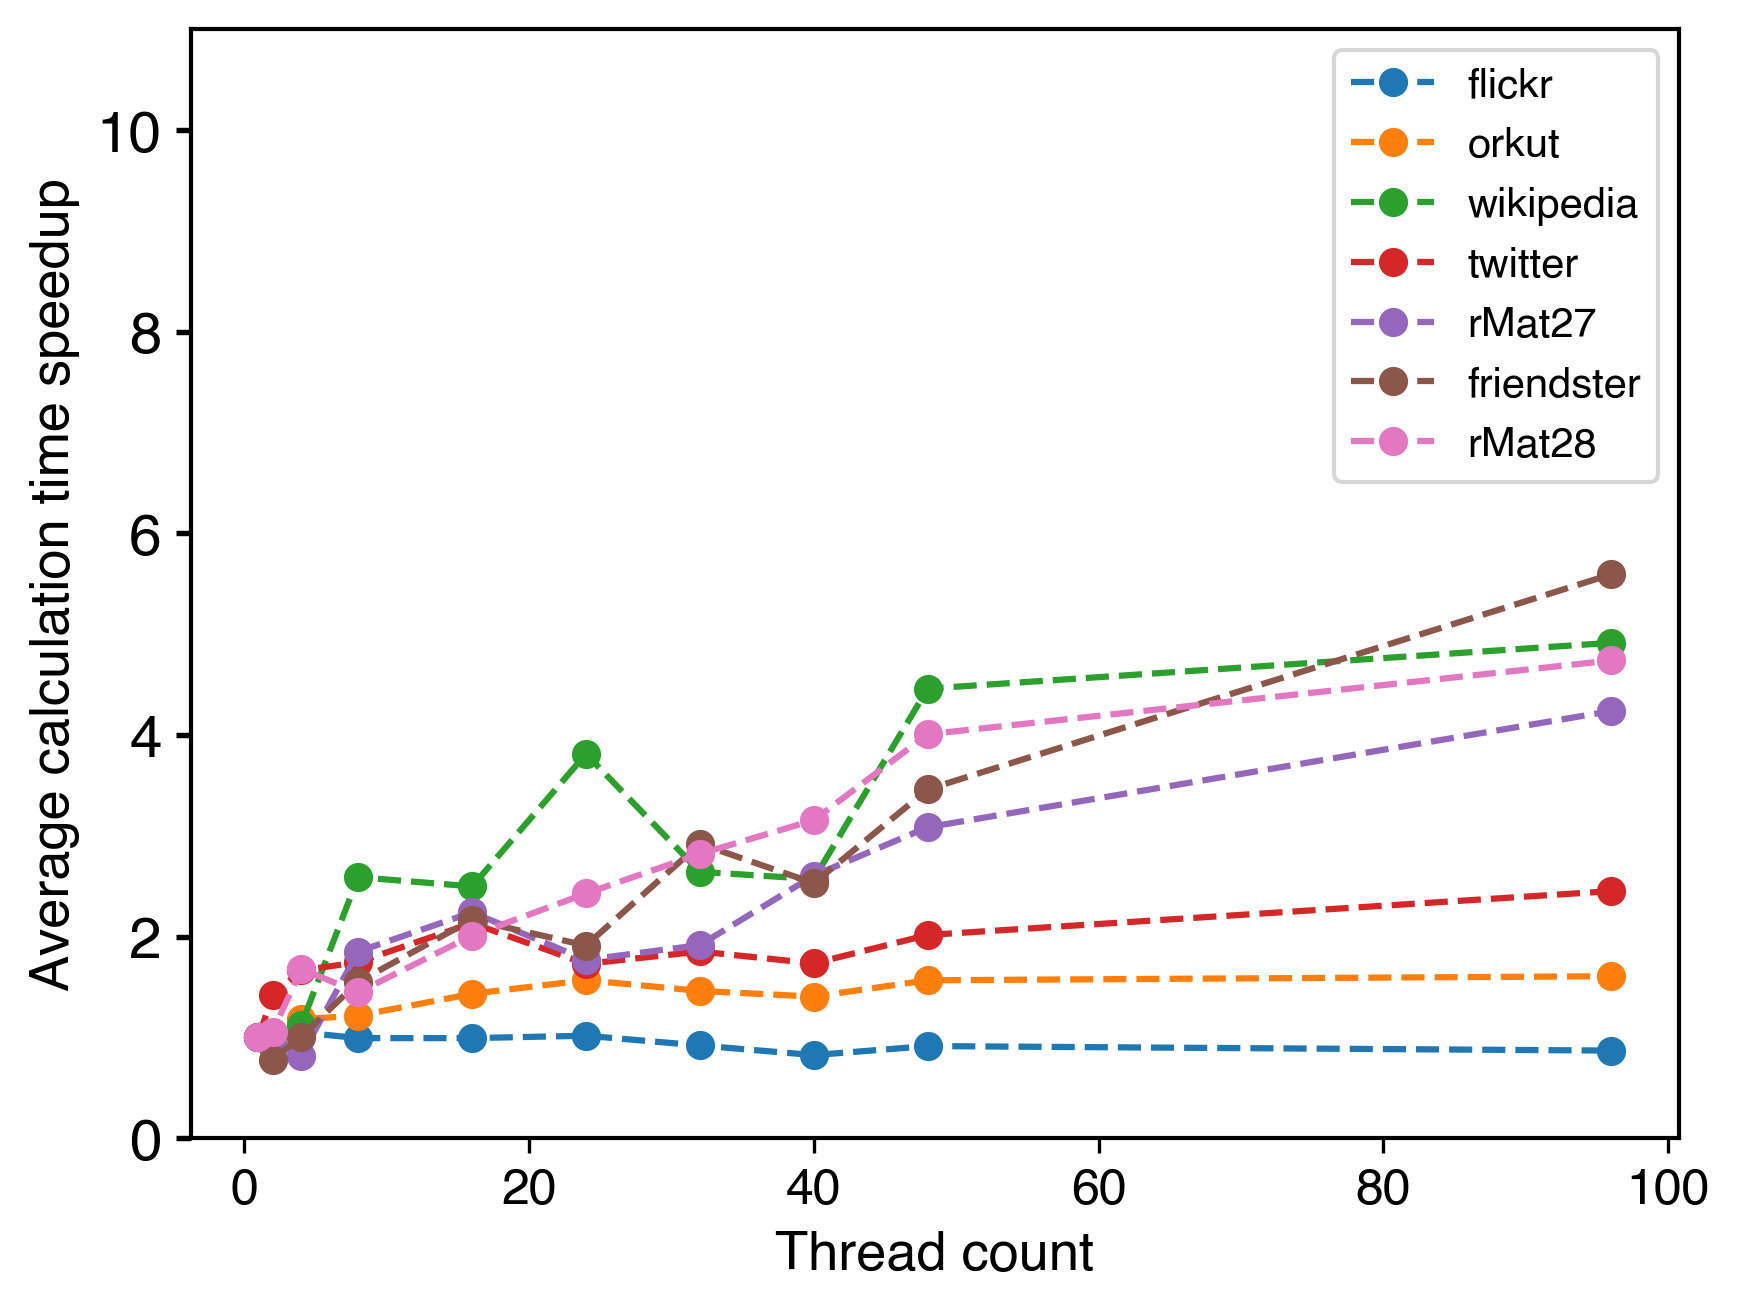
\includegraphics[width=\linewidth]{../../plots/singleNodeBFSGaloisThreads.png}
		\caption{Breadth-first search}
		\label{fig:singleNodeBFSGaloisThreads}
	\end{subfigure}
	\caption{Calculation time speedup with increasing thread count for Galois Single-source Shortest-paths and Breadth-first search algorithms.}
\end{figure}



\begin{figure}
	\begin{subfigure}{\columnwidth}
		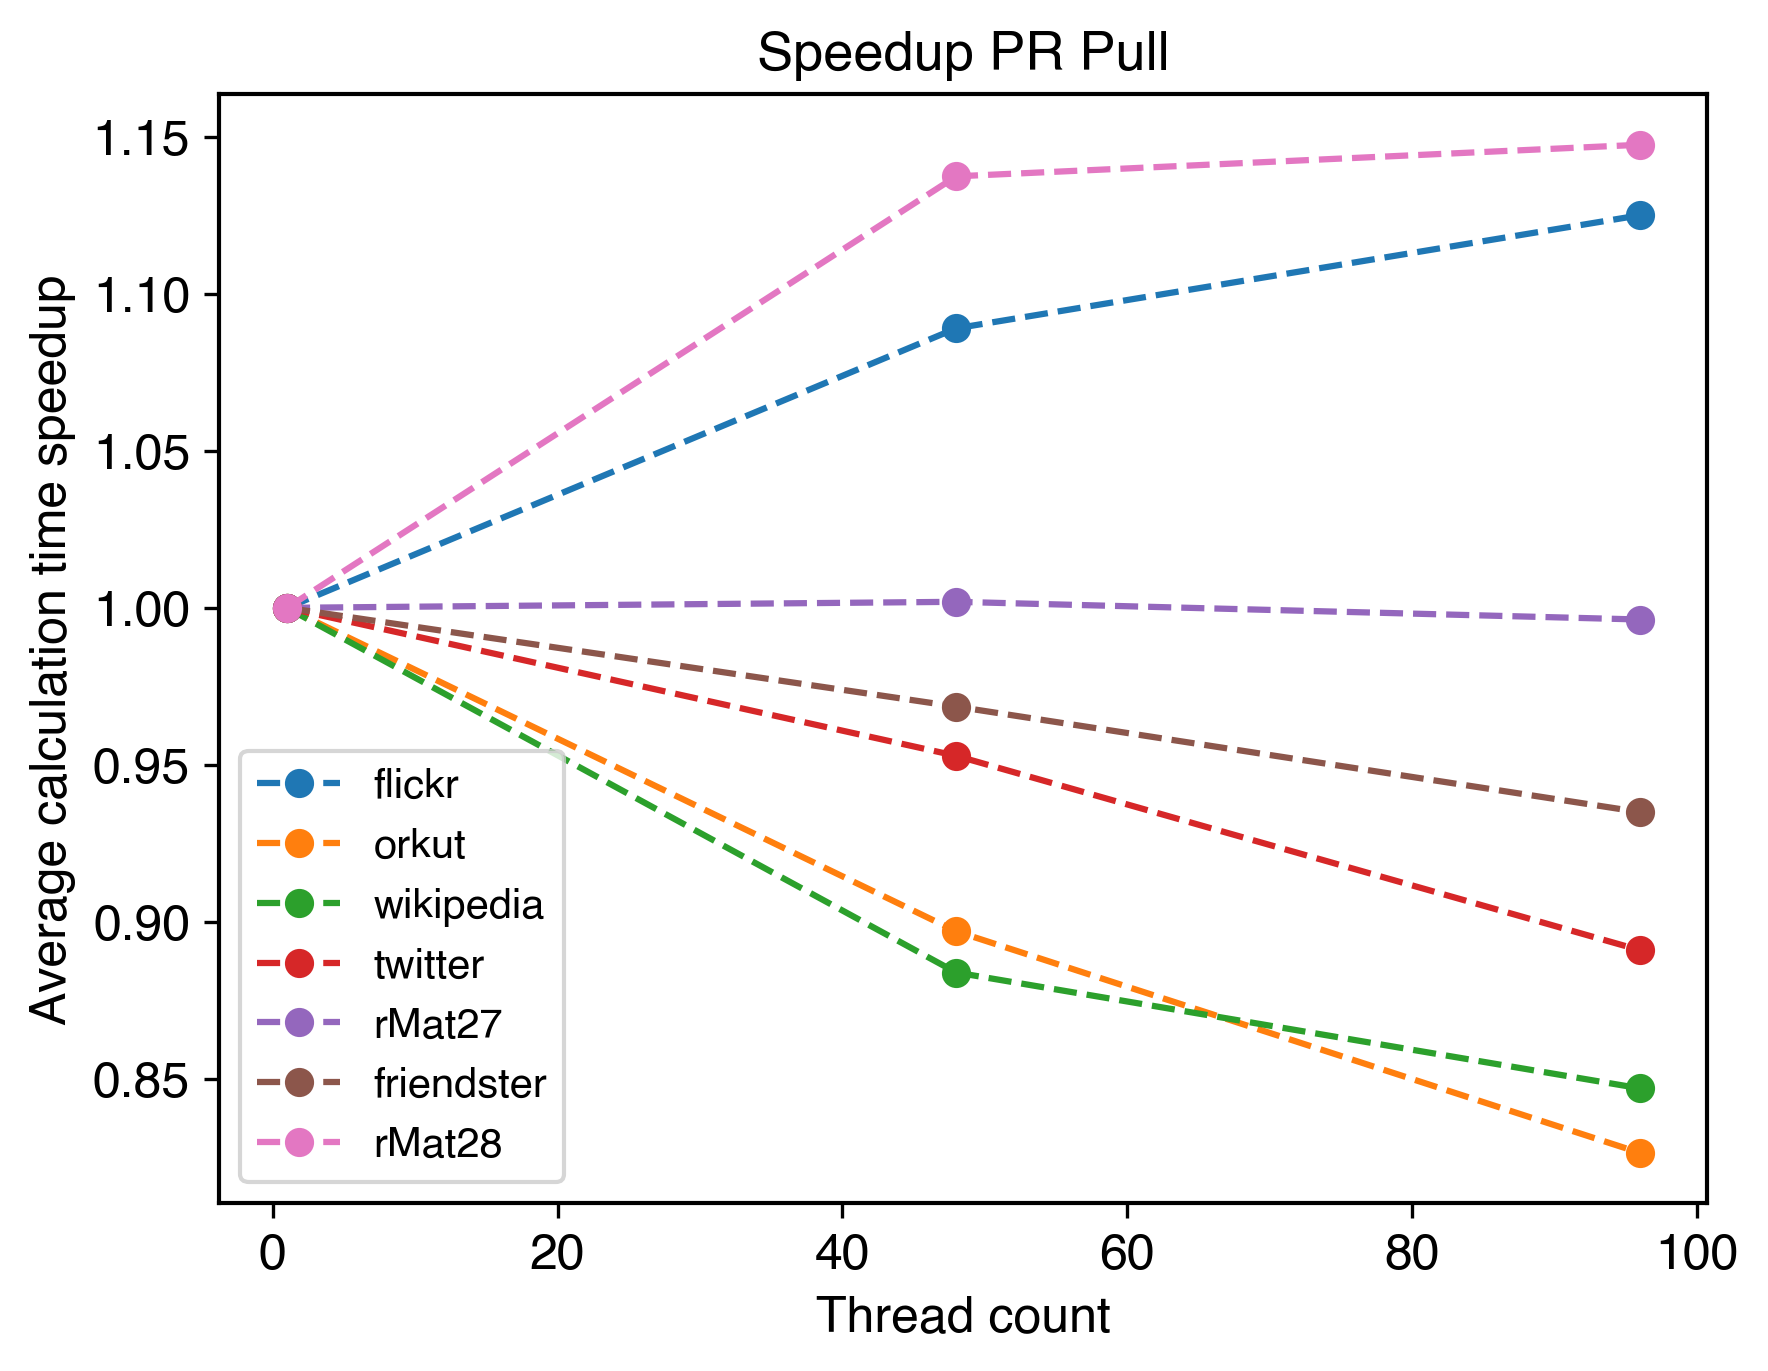
\includegraphics[width=\columnwidth]{../../plots/singleNodePRPullGaloisThreads.png}
		\caption{PageRank Pull}
		\label{fig:singleNodePRPullGaloisThreads}
	\end{subfigure}
	\begin{subfigure}{\columnwidth}
		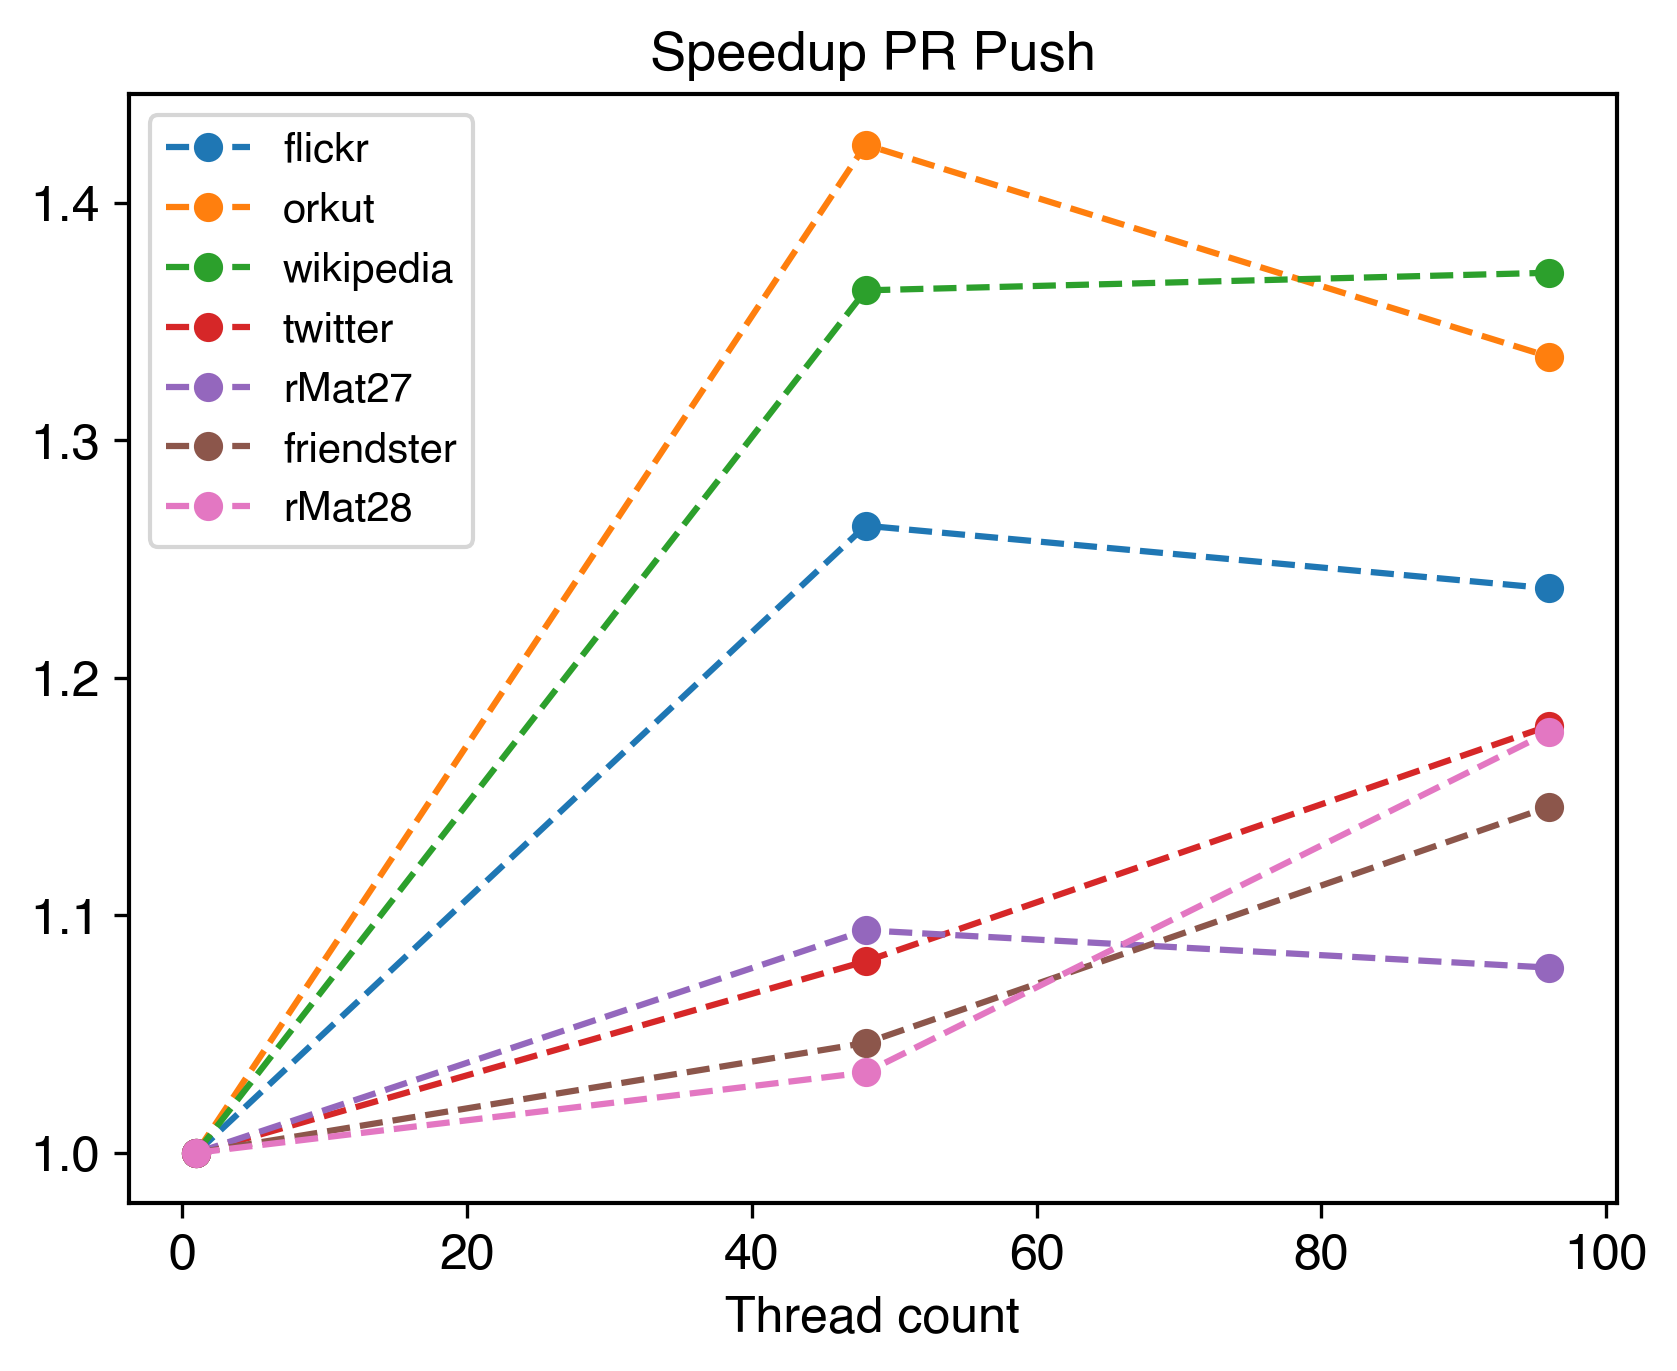
\includegraphics[width=\columnwidth]{../../plots/singleNodePRPushGaloisThreads.png}
		\caption{PageRank Push}
		\label{fig:singleNodePRPushGaloisThreads}
	\end{subfigure}
	\caption{Calculation time speedup with increasing thread count for Galois PageRank Push and Pull algorithms.}
\end{figure}





\subsection{Execution times and overhead}



\begin{figure}
	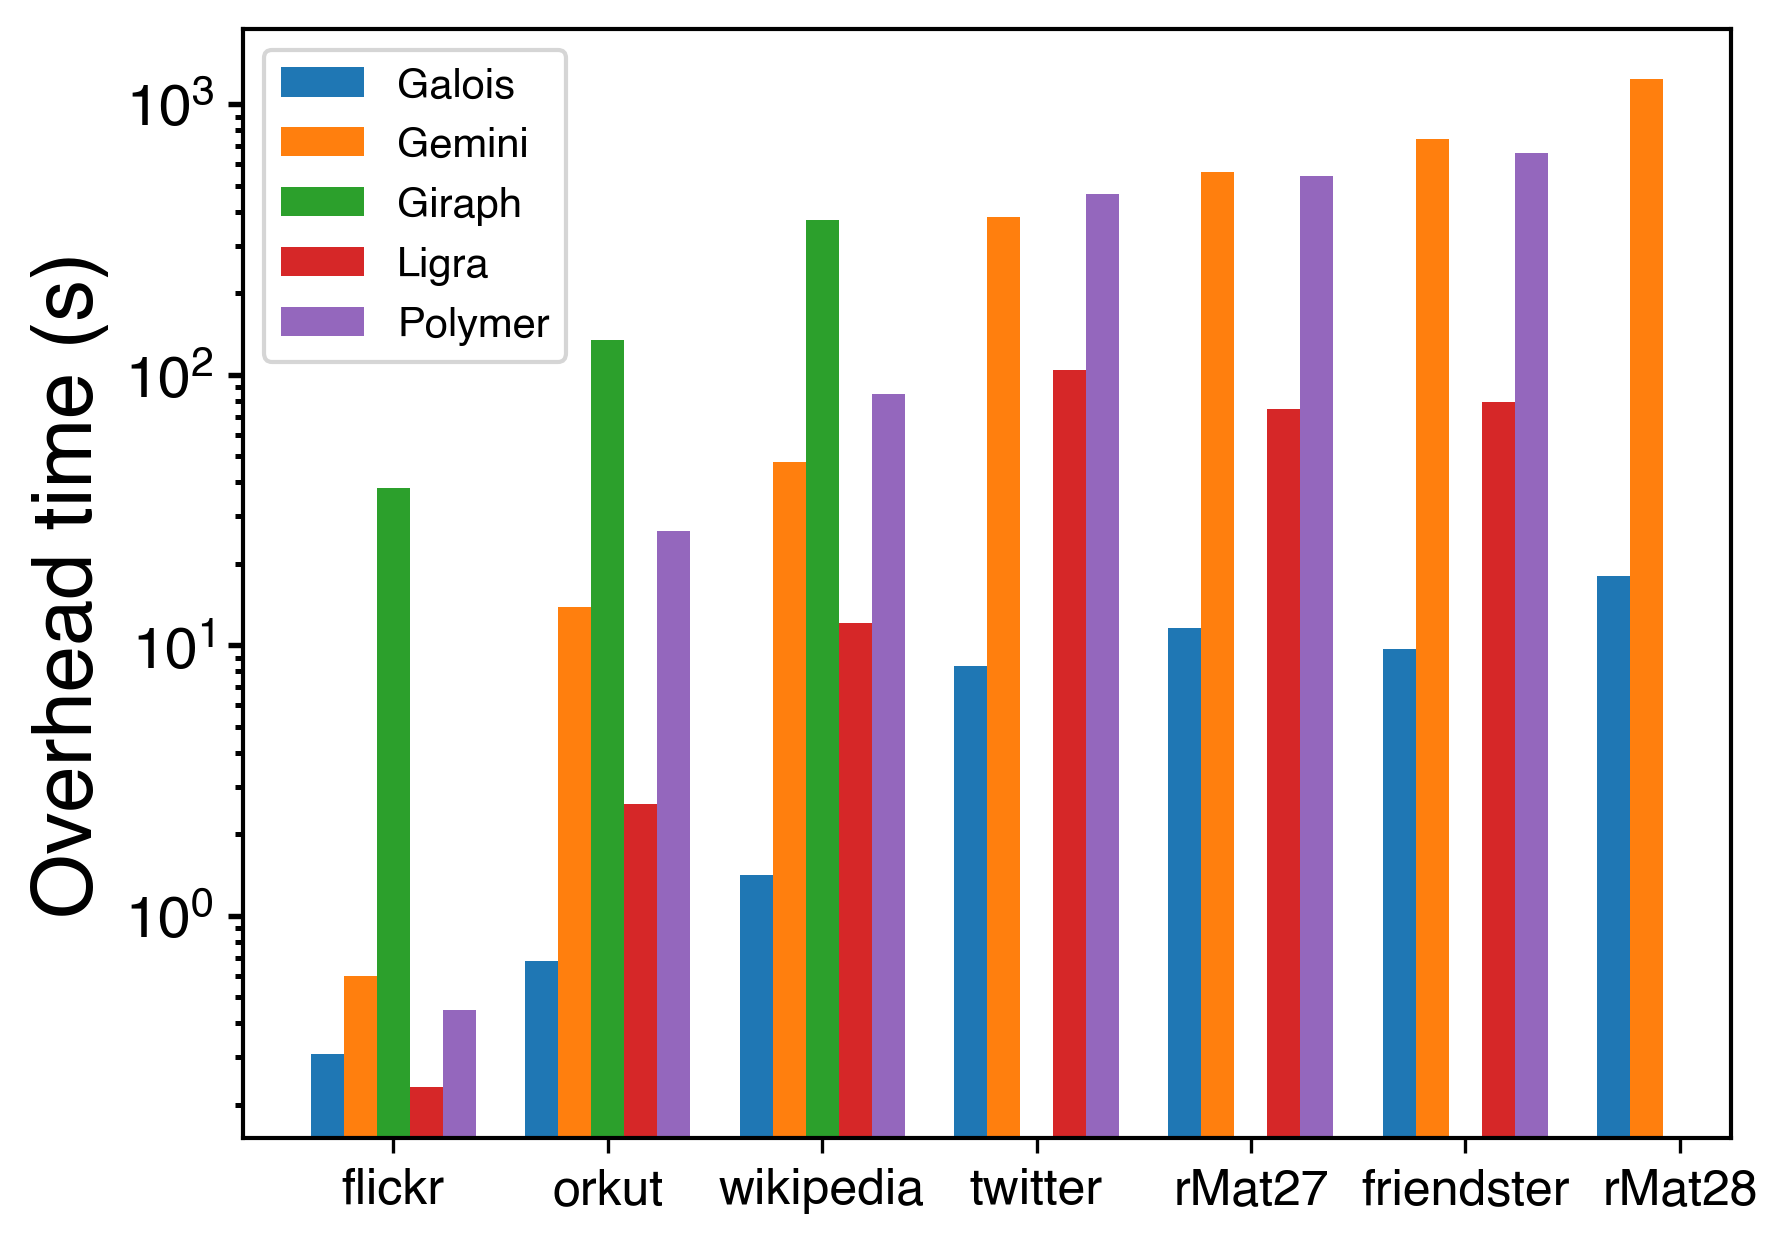
\includegraphics[width=\columnwidth]{../../plots/singleNodeSSSP_overheadTime.png}
	\caption{Overhead SSSP single node}
	\label{fig:singleNodeSSSP_overhead}
\end{figure}



\begin{figure}
	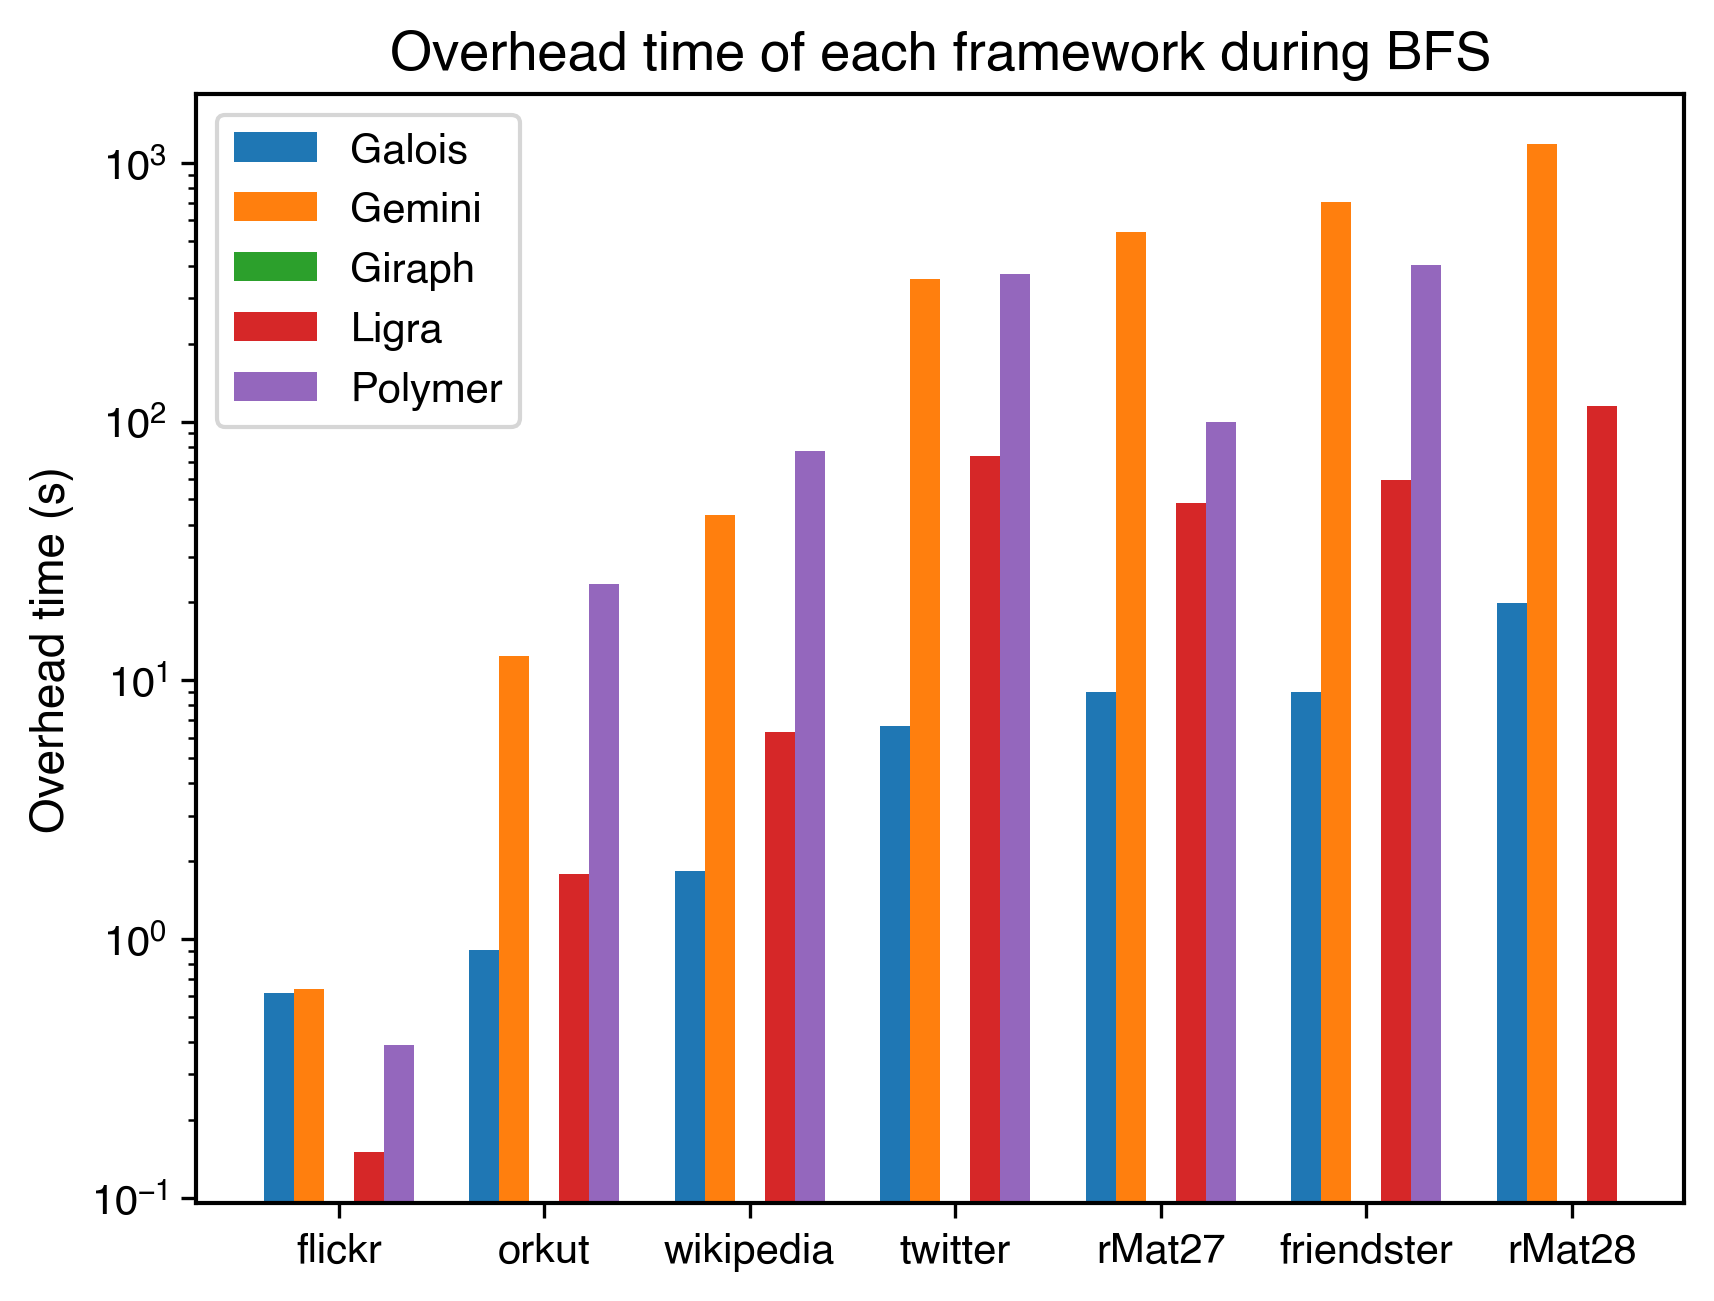
\includegraphics[width=\columnwidth]{../../plots/singleNodeBFS_overheadTime.png}
	\caption{Overhead BFS single node}
	\label{fig:singleNodeBFS_overhead}
\end{figure}



hier erhoffe ich mir einen Vergleich der Ladezeiten und erwarte, dass Systeme wie Giraph, die erstmal auf irgendwas warten schlecht abschneiden.
Aber vielleicht ist auch die setup time bei gleichen frameworks zwischen verteilt und shared memory ganz interessant zu vergleichen. 
